\chapter{Threefold Data}
\label{appendix1}
\renewcommand{\thefootnote}{\fnsymbol{footnote}} 
\setcounter{footnote}{0}
In this Appendix we...

Key:

{\setlength{\parindent}{0pt}
\newpage
%
%
%
%
%
%
%
\begin{tabularx}{\textwidth}{rlrl}
\toprule
\textbf{Name:} & \ 2.30 \hspace{0.3\textwidth} & \textbf{Description:} & Blow up of $Q$ in a line\\
\midrule
\textbf{$\sigma$}: & {\small $\begin{pmatrix} -1 & 0 \\ 0 & 1 \end{pmatrix}$ } & $ R(X) = 23/29$ , & $\xi \sim (0,0.51489)$
\end{tabularx}

\begin{figure}[H]
\centering


\label{fig:data230b}
\resizebox{0.9\linewidth}{!}{
\begin{subfigure}[b]{0.30\textwidth}
\centering
  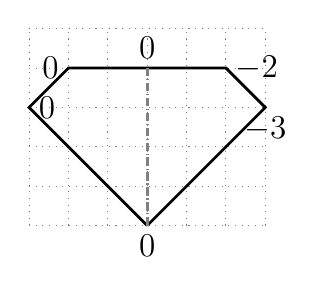
\begin{tikzpicture}[scale=0.5]
   	 \draw[dotted,step=1,gray,] (-3,-3) grid (3,2); \draw[line width = 1pt] (0,-3) --
     (-3,0) -- (-2,1)--(2,1)--
 	 (3,0)--(0,-3); \draw[densely dashdotted, gray, line width = 1.2pt] (0,-3) -- (0,1);
 	 \node at (0,-3) [below] {\large{$0$}};
 	 \node at (-3,0) [right] {\large{$0$}};
 	 \node at (-2,1) [left] {\large{$0$}};
 	 \node at (2,1) [right] {\large{$-2$}};
 	 \node at (3,0) [below] {\large{$-3$}};
 	 \node at (0,1) [above] {\large{$0$}};
	\end{tikzpicture}
	\caption*{$\Phi_0$}
\end{subfigure}
\begin{subfigure}[b]{0.30\textwidth}
	\centering
 	 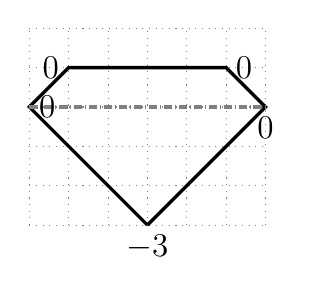
\begin{tikzpicture}[scale=0.5]
 	   \draw[dotted,step=1,gray] (-3,-3) grid (3,2); \draw[line width = 1.2pt] (0,-3) --
 	   (-3,0) -- (-2,1)--(2,1)--
 	   (3,0)--(0,-3); \draw[densely dashdotted, gray,line width = 1.2pt] (-3,0) -- (3,0);
 	 \node at (0,-3) [below] {\large{$-3$}};
 	 \node at (-3,0) [right] {\large{$0$}};
 	 \node at (-2,1) [left] {\large{$0$}};
 	 \node at (2,1) [right] {\large{$0$}};
 	 \node at (3,0) [below] {\large{$0$}};
	\end{tikzpicture}
	\caption*{$\Phi_1$}
\end{subfigure}
\begin{subfigure}[b]{0.30\textwidth}
	\centering
 	 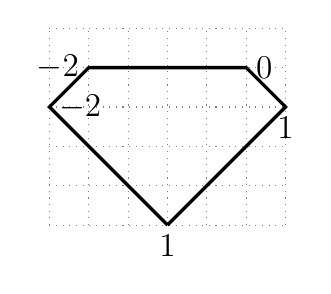
\begin{tikzpicture}[scale=0.5]
 	   \draw[dotted,step=1,gray] (-3,-3) grid (3,2); \draw[line width = 1.2pt] (0,-3) --
 	   (-3,0) -- (-2,1)--(2,1)--
 	   (3,0)--(0,-3);
 	 \node at (0,-3) [below] {\large{$1$}};
 	 \node at (-3,0) [right] {\large{$-2$}};
 	 \node at (-2,1) [left] {\large{$-2$}};
 	 \node at (2,1) [right] {\large{$0$}};
 	 \node at (3,0) [below] {\large{$1$}};
	\end{tikzpicture}
	\caption*{$\Phi_\infty$}
\end{subfigure}
\begin{subfigure}[b]{0.40\textwidth}
	\centering
 	 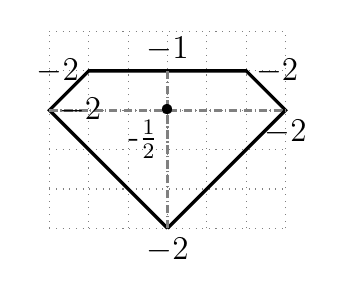
\begin{tikzpicture}[scale=0.5]
 	   \draw[dotted,step=1,gray] (-3,-3) grid (3,2); \draw[line width = 1.2pt] (0,-3) --
 	   (-3,0) -- (-2,1)--(2,1)--
 	   (3,0)--(0,-3); \draw[densely dashdotted, gray,line width = 1.2pt] (-3,0) -- (3,0); \draw[densely dashdotted, gray,line width = 1.2pt] (0,-3) -- (0,1) ;
 	 \node at (0,-3) [below] {\large{$-2$}};
 	 \node at (-3,0) [right] {\large{$-2$}};
 	 \node at (-2,1) [left] {\large{$-2$}};
 	 \node at (2,1) [right] {\large{$-2$}};
 	 \node at (3,0) [below] {\large{$-2$}};
 	 \node at (0,0) [below left] {\large{-$\frac{1}{2}$}};
 	 \node at (0,1) [above] {\large{$-1$}};
 	 \draw (0,0) node {\textbullet};
	\end{tikzpicture}
	\caption*{$\deg \Phi $}
\end{subfigure}
}
\end{figure}
\begin{tabularx}{\textwidth}{|c|c|c}
\toprule
\(y\) & \(\text{Vert}(\Delta_y)\) & \(n_y\) \\
\midrule
\(0\) & \begin{tabular}{l} \((-3,0,1),(-2,1,1),(2,1,-1),\) \\ \hspace{1cm} \((3,0,-2),(0,-3,1),(0,1,1)\) \end{tabular} & \((a,b,c)\) \\ \midrule
\(1\) & \begin{tabular}{l} \((-3,0,1),(-2,1,1),(0,1,0),\) \\ \hspace{1cm} \((2,1,1),(3,0,1),(0,-3,-2)\) \end{tabular} & \((a,b,c)\) \\ \midrule
\(\infty\) & \begin{tabular}{l} \((-3,0,-1),(-2,1,-1),(2,1,1),\) \\ \hspace{1cm} \((3,0,2),(0,-3,2),(0,0,-1),(0,1,-1)\) \end{tabular} & \((a,b,c)\) \\
\midrule
\end{tabularx}
\begin{align*}
g(\xi) &= \frac{1}{\xi_{2}^{4}}\cdot\left({\left(2 \, \xi_{2}^{3} - 3 \, \xi_{2} - 3\right)} e^{\left(4 \, \xi_{2}\right)} + 12 \, \xi_{2} e^{\left(3 \, \xi_{2}\right)} + 3 \, \xi_{2} + 3\right) e^{\left(-3 \, \xi_{2}\right)}
\end{align*}
\begin{tabularx}{\textwidth}{|c|c|c}
\toprule
\(y\) & \( h_y(\xi_2)\) & \( h_y(\xi_2) \in\) \\
\midrule
\(0\) & \begin{tabular}{l} \(\frac{1}{3\xi_2^{4}} \cdot
 ( \ (2   \xi_2^{3} - 3   \xi_2 - 3) e^{4   \xi_2} \)   \\ \hspace{2cm} \(+12 \xi_2 e^{3 \xi_2} + 3 \xi_2 + 3 \ ) e^{-3 \xi_2}\) \end{tabular} & \((1.087,1.458)\) \\ \midrule
\(1\) & \begin{tabular}{l} \(\frac{1}{3\xi_2^{4}} \cdot
 ( \ (2   \xi_2^{3} - 3   \xi_2 - 3) e^{4   \xi_2} \)   \\ \hspace{2cm} \(+12 \xi_2 e^{3 \xi_2} + 3 \xi_2 + 3 \ ) e^{-3 \xi_2}\) \end{tabular} & \((2.178,2.470)\) \\ \midrule
\(\infty\) & \begin{tabular}{l} \(\frac{1}{3\xi_2^{4}} \cdot
 ( \ (2   \xi_2^{3} - 3   \xi_2 - 3) e^{4   \xi_2} \)   \\ \hspace{2cm} \(+12 \xi_2 e^{3 \xi_2} + 3 \xi_2 + 3 \ ) e^{-3 \xi_2}\) \end{tabular} & \((0.446,0.827)\) \\ \midrule
\(\notin \{0,1,\infty\}\) & \begin{tabular}{l} \(\frac{1}{3\xi_2^{4}} \cdot
 ( \ (2   \xi_2^{3} - 3   \xi_2 - 3) e^{4   \xi_2} \)   \\ \hspace{2cm} \(+12 \xi_2 e^{3 \xi_2} + 3 \xi_2 + 3 \ ) e^{-3 \xi_2}\) \end{tabular} & \((4.151,4.309)\) \\
 \bottomrule
\end{tabularx}
\newpage
%
%
%
%
%
%
%
\begin{tabularx}{\textwidth}{rlrl}
\toprule
\textbf{Name:} & \ 2.31 \hspace{0.3\textwidth} & \textbf{Description:} & Blow up of $Q$ in a line\\
\midrule
\textbf{$\sigma$}: & {\small $\begin{pmatrix} -1 & 0 \\ 0 & 1 \end{pmatrix}$ } & $ R(X) = 23/29$ , & $\xi \sim (0,0.51489)$
\end{tabularx}

\begin{figure}[H]
\centering
\label{fig:data231}
\resizebox{0.9\linewidth}{!}{
\begin{subfigure}[b]{0.30\textwidth}
\centering
  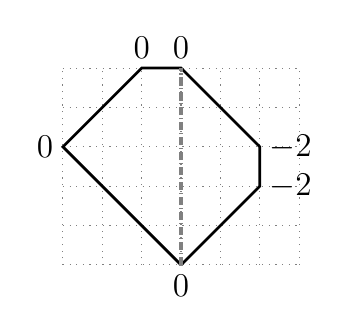
\begin{tikzpicture}[scale=0.5]
   	 \draw[dotted,step=1,gray,] (-3,-3) grid (3,2); \draw[line width = 1pt] (0,-3) --
     (-3,0) -- (-1,2)--(0,2)--
 	 (2,0)--(2,-1) -- (0,-3); \draw[densely dashdotted, gray, line width = 1.2pt] (0,-3) -- (0,2);
 	 \node at (0,-3) [below] {\large{$0$}};
 	 \node at (-3,0) [left] {\large{$0$}};
 	 \node at (-1,2) [above] {\large{$0$}};
 	 \node at (0,2) [above] {\large{$0$}};
 	 \node at (2,0) [right] {\large{$-2$}};
 	 \node at (2,-1) [right] {\large{$-2$}};
	\end{tikzpicture}
	\caption*{$\Phi_0$}
\end{subfigure}
\begin{subfigure}[b]{0.30\textwidth}
	\centering
 	 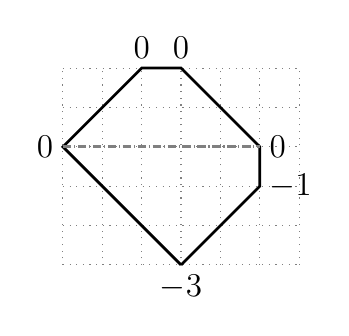
\begin{tikzpicture}[scale=0.5]
 	   \draw[dotted,step=1,gray] (-3,-3) grid (3,2); \draw[line width = 1pt] (0,-3) --
     (-3,0) -- (-1,2)--(0,2)--
 	 (2,0)--(2,-1) -- (0,-3); \draw[densely dashdotted, gray,line width = 1.2pt] (-3,0) -- (2,0);
 	 \node at (0,-3) [below] {\large{$-3$}};
 	 \node at (-3,0) [left] {\large{$0$}};
 	 \node at (-1,2) [above] {\large{$0$}};
 	 \node at (0,2) [above] {\large{$0$}};
 	 \node at (2,0) [right] {\large{$0$}};
 	 \node at (2,-1) [right] {\large{$-1$}};
	\end{tikzpicture}
	\caption*{$\Phi_1$}
\end{subfigure}
\begin{subfigure}[b]{0.30\textwidth}
	\centering
 	 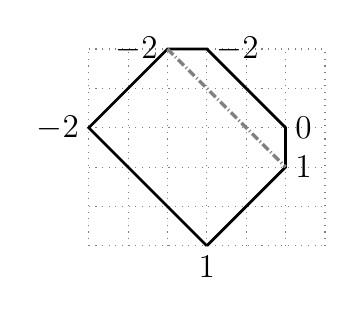
\begin{tikzpicture}[scale=0.5]
 	   \draw[dotted,step=1,gray] (-3,-3) grid (3,2); \draw[line width = 1pt] (0,-3) --
     (-3,0) -- (-1,2)--(0,2)--
 	 (2,0)--(2,-1) -- (0,-3); \draw[densely dashdotted, gray,line width = 1.2pt] (-1,2) -- (2,-1);
 	 \node at (0,-3) [below] {\large{$1$}};
 	 \node at (-3,0) [left] {\large{$-2$}};
 	 \node at (-1,2) [left] {\large{$-2$}};
 	 \node at (0,2) [right] {\large{$-2$}};
 	 \node at (2,0) [right] {\large{$0$}};
 	 \node at (2,-1) [right] {\large{$1$}};
	\end{tikzpicture}
	\caption*{$\Phi_\infty$}
\end{subfigure}
\begin{subfigure}[b]{0.40\textwidth}
	\centering
 	 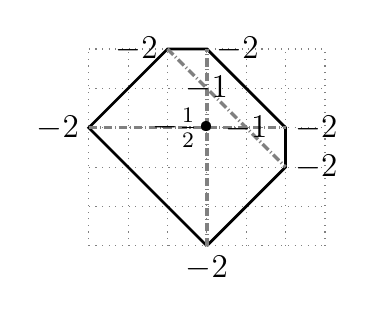
\begin{tikzpicture}[scale=0.5]
 	   \draw[dotted,step=1,gray] (-3,-3) grid (3,2); \draw[line width = 1pt] (0,-3) --
     (-3,0) -- (-1,2)--(0,2)--
 	 (2,0)--(2,-1) -- (0,-3); \draw[densely dashdotted, gray, line width = 1.2pt] (0,-3) -- (0,2);  \draw[densely dashdotted, gray,line width = 1.2pt] (-3,0) -- (2,0); \draw[densely dashdotted, gray,line width = 1.2pt] (-1,2) -- (2,-1);
 	 \node at (0,-3) [below] {\large{$-2$}};
 	 \node at (-3,0) [left] {\large{$-2$}};
 	 \node at (-1,2) [left] {\large{$-2$}};
 	 \node at (0,2) [right] {\large{$-2$}};
 	 \node at (2,0) [right] {\large{$-2$}};
 	 \node at (2,-1) [right] {\large{$-2$}};
 	 \node at (1,0) {\large{$-1$}};
 	 \node at (0,1) {\large{$-1$}};
 	 \node at (0,0) [left] {\large{$-\frac{1}{2}$}};
 	 \draw (0,0) node {\textbullet};
	\end{tikzpicture}
	\caption*{$\deg \Phi $}
\end{subfigure}
}
\end{figure}
\begin{tabularx}{\textwidth}{|c|c|c}
\toprule
\(y\) & \(\text{Vert}(\Delta_y)\) & \(n_y\) \\
\midrule
\(0\) & \begin{tabular}{l} \((-3,0,1),(-2,1,1),(2,1,-1),\) \\ \hspace{1cm} \((3,0,-2),(0,-3,1),(0,1,1)\) \end{tabular} & \((a,b,c)\) \\ \midrule
\(1\) & \begin{tabular}{l} \((-3,0,1),(-2,1,1),(0,1,0),\) \\ \hspace{1cm} \((2,1,1),(3,0,1),(0,-3,-2)\) \end{tabular} & \((a,b,c)\) \\ \midrule
\(\infty\) & \begin{tabular}{l} \((-3,0,-1),(-2,1,-1),(2,1,1),\) \\ \hspace{1cm} \((3,0,2),(0,-3,2),(0,0,-1),(0,1,-1)\) \end{tabular} & \((a,b,c)\) \\
\midrule
\end{tabularx}
\begin{align*}
g(\xi) &= \frac{1}{\xi_{2}^{4}}\cdot\left({\left(2 \, \xi_{2}^{3} - 3 \, \xi_{2} - 3\right)} e^{\left(4 \, \xi_{2}\right)} + 12 \, \xi_{2} e^{\left(3 \, \xi_{2}\right)} + 3 \, \xi_{2} + 3\right) e^{\left(-3 \, \xi_{2}\right)}
\end{align*}
\begin{tabularx}{\textwidth}{|c|c|c}
\toprule
\(y\) & \( h_y(\xi_2)\) & \( h_y(\xi_2) \in\) \\
\midrule
\(0\) & \begin{tabular}{l} \(\frac{1}{3\xi_2^{4}} \cdot
 ( \ (2   \xi_2^{3} - 3   \xi_2 - 3) e^{4   \xi_2} \)   \\ \hspace{2cm} \(+12 \xi_2 e^{3 \xi_2} + 3 \xi_2 + 3 \ ) e^{-3 \xi_2}\) \end{tabular} & \((1.087,1.458)\) \\ \midrule
\(1\) & \begin{tabular}{l} \(\frac{1}{3\xi_2^{4}} \cdot
 ( \ (2   \xi_2^{3} - 3   \xi_2 - 3) e^{4   \xi_2} \)   \\ \hspace{2cm} \(+12 \xi_2 e^{3 \xi_2} + 3 \xi_2 + 3 \ ) e^{-3 \xi_2}\) \end{tabular} & \((2.178,2.470)\) \\ \midrule
\(\infty\) & \begin{tabular}{l} \(\frac{1}{3\xi_2^{4}} \cdot
 ( \ (2   \xi_2^{3} - 3   \xi_2 - 3) e^{4   \xi_2} \)   \\ \hspace{2cm} \(+12 \xi_2 e^{3 \xi_2} + 3 \xi_2 + 3 \ ) e^{-3 \xi_2}\) \end{tabular} & \((0.446,0.827)\) \\ \midrule
\(\notin \{0,1,\infty\}\) & \begin{tabular}{l} \(\frac{1}{3\xi_2^{4}} \cdot
 ( \ (2   \xi_2^{3} - 3   \xi_2 - 3) e^{4   \xi_2} \)   \\ \hspace{2cm} \(+12 \xi_2 e^{3 \xi_2} + 3 \xi_2 + 3 \ ) e^{-3 \xi_2}\) \end{tabular} & \((4.151,4.309)\) \\
 \bottomrule
\end{tabularx}
\newpage
%
%
%
%
%
%
%
%
\begin{tabularx}{\textwidth}{rlrl}
\toprule
\textbf{Name:} & \ 2.31 \hspace{0.3\textwidth} & \textbf{Description:} & Blow up of $Q$ in a line\\
\midrule
\textbf{$\sigma$}: & {\small $\begin{pmatrix} -1 & 0 \\ 0 & 1 \end{pmatrix}$ } & $ R(X) = 23/29$ , & $\xi \sim (0,0.51489)$
\end{tabularx}

\begin{figure}[h]
\centering
\label{fig:data38*}
\resizebox{0.9\linewidth}{!}{
\begin{subfigure}[b]{0.30\textwidth}
\centering
  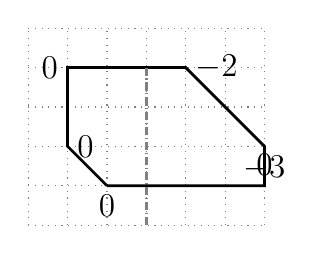
\begin{tikzpicture}[scale=0.5]
   	 \draw[dotted,step=1,gray,] (-3,-3) grid (3,2); \draw[line width = 1pt] (-1,-2) --
     (-2,-1) -- (-2,1)--(1,1)--
 	 (3,-1)--(3,-2) -- (-1,-2); \draw[densely dashdotted, gray, line width = 1.2pt] (0,-3) -- (0,1);
 	 \node at (-1,-2) [below] {\large{$0$}};
 	 \node at (-2,-1) [right] {\large{$0$}};
 	 \node at (-2,1) [left] {\large{$0$}};
 	 \node at (1,1) [right] {\large{$-2$}};
 	 \node at (3,-1) [below] {\large{$-3$}};
 	 \node at (3,-2) [above] {\large{$0$}};
	\end{tikzpicture}
	\caption*{$\Phi_0$}
\end{subfigure}
\begin{subfigure}[b]{0.30\textwidth}
	\centering
 	 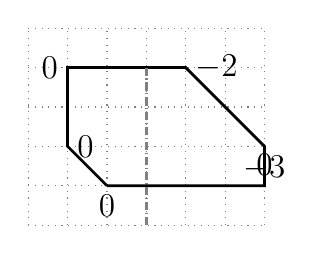
\begin{tikzpicture}[scale=0.5]
   	 \draw[dotted,step=1,gray,] (-3,-3) grid (3,2); \draw[line width = 1pt] (-1,-2) --
     (-2,-1) -- (-2,1)--(1,1)-- (3,-1)--(3,-2) -- (-1,-2); \draw[densely dashdotted, gray, line width = 1.2pt] (0,-3) -- (0,1);
 	 \node at (-1,-2) [below] {\large{$0$}};
 	 \node at (-2,-1) [right] {\large{$0$}};
 	 \node at (-2,1) [left] {\large{$0$}};
 	 \node at (1,1) [right] {\large{$-2$}};
 	 \node at (3,-1) [below] {\large{$-3$}};
 	 \node at (3,-2) [above] {\large{$0$}};
	\end{tikzpicture}
	\caption*{$\Phi_1$}
\end{subfigure}
\begin{subfigure}[b]{0.30\textwidth}
	\centering
 	 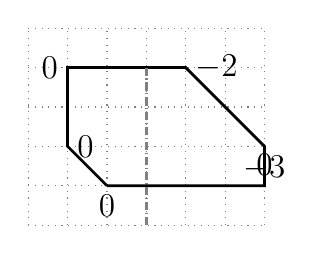
\begin{tikzpicture}[scale=0.5]
   	 \draw[dotted,step=1,gray,] (-3,-3) grid (3,2); \draw[line width = 1pt] (-1,-2) --
     (-2,-1) -- (-2,1)--(1,1)-- (3,-1)--(3,-2) -- (-1,-2); \draw[densely dashdotted, gray, line width = 1.2pt] (0,-3) -- (0,1);
 	 \node at (-1,-2) [below] {\large{$0$}};
 	 \node at (-2,-1) [right] {\large{$0$}};
 	 \node at (-2,1) [left] {\large{$0$}};
 	 \node at (1,1) [right] {\large{$-2$}};
 	 \node at (3,-1) [below] {\large{$-3$}};
 	 \node at (3,-2) [above] {\large{$0$}};
	\end{tikzpicture}
	\caption*{$\Phi_\infty$}
\end{subfigure}
\begin{subfigure}[b]{0.40\textwidth}
	\centering
 	 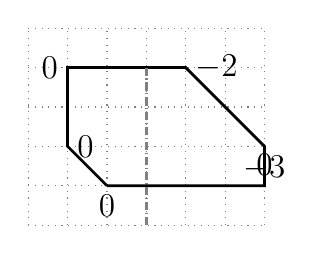
\begin{tikzpicture}[scale=0.5]
   	 \draw[dotted,step=1,gray,] (-3,-3) grid (3,2); \draw[line width = 1pt] (-1,-2) --
     (-2,-1) -- (-2,1)--(1,1)-- (3,-1)--(3,-2) -- (-1,-2); \draw[densely dashdotted, gray, line width = 1.2pt] (0,-3) -- (0,1);
 	 \node at (-1,-2) [below] {\large{$0$}};
 	 \node at (-2,-1) [right] {\large{$0$}};
 	 \node at (-2,1) [left] {\large{$0$}};
 	 \node at (1,1) [right] {\large{$-2$}};
 	 \node at (3,-1) [below] {\large{$-3$}};
 	 \node at (3,-2) [above] {\large{$0$}};
	\end{tikzpicture}
	\caption*{$\deg \Phi $}
\end{subfigure}
}
\end{figure}
\begin{tabularx}{\textwidth}{|c|c|c}
\toprule
\(y\) & \(\text{Vert}(\Delta_y)\) & \(n_y\) \\
\midrule
\(0\) & \begin{tabular}{l} \((-3,0,1),(-2,1,1),(2,1,-1),\) \\ \hspace{1cm} \((3,0,-2),(0,-3,1),(0,1,1)\) \end{tabular} & \((a,b,c)\) \\ \midrule
\(1\) & \begin{tabular}{l} \((-3,0,1),(-2,1,1),(0,1,0),\) \\ \hspace{1cm} \((2,1,1),(3,0,1),(0,-3,-2)\) \end{tabular} & \((a,b,c)\) \\ \midrule
\(\infty\) & \begin{tabular}{l} \((-3,0,-1),(-2,1,-1),(2,1,1),\) \\ \hspace{1cm} \((3,0,2),(0,-3,2),(0,0,-1),(0,1,-1)\) \end{tabular} & \((a,b,c)\) \\
\midrule
\end{tabularx}
\begin{align*}
g(\xi) &= \frac{1}{\xi_{2}^{4}}\cdot\left({\left(2 \, \xi_{2}^{3} - 3 \, \xi_{2} - 3\right)} e^{\left(4 \, \xi_{2}\right)} + 12 \, \xi_{2} e^{\left(3 \, \xi_{2}\right)} + 3 \, \xi_{2} + 3\right) e^{\left(-3 \, \xi_{2}\right)}
\end{align*}
\begin{tabularx}{\textwidth}{|c|c|c}
\toprule
\(y\) & \( h_y(\xi_2)\) & \( h_y(\xi_2) \in\) \\
\midrule
\(0\) & \begin{tabular}{l} \(\frac{1}{3\xi_2^{4}} \cdot
 ( \ (2   \xi_2^{3} - 3   \xi_2 - 3) e^{4   \xi_2} \)   \\ \hspace{2cm} \(+12 \xi_2 e^{3 \xi_2} + 3 \xi_2 + 3 \ ) e^{-3 \xi_2}\) \end{tabular} & \((1.087,1.458)\) \\ \midrule
\(1\) & \begin{tabular}{l} \(\frac{1}{3\xi_2^{4}} \cdot
 ( \ (2   \xi_2^{3} - 3   \xi_2 - 3) e^{4   \xi_2} \)   \\ \hspace{2cm} \(+12 \xi_2 e^{3 \xi_2} + 3 \xi_2 + 3 \ ) e^{-3 \xi_2}\) \end{tabular} & \((2.178,2.470)\) \\ \midrule
\(\infty\) & \begin{tabular}{l} \(\frac{1}{3\xi_2^{4}} \cdot
 ( \ (2   \xi_2^{3} - 3   \xi_2 - 3) e^{4   \xi_2} \)   \\ \hspace{2cm} \(+12 \xi_2 e^{3 \xi_2} + 3 \xi_2 + 3 \ ) e^{-3 \xi_2}\) \end{tabular} & \((0.446,0.827)\) \\ \midrule
\(\notin \{0,1,\infty\}\) & \begin{tabular}{l} \(\frac{1}{3\xi_2^{4}} \cdot
 ( \ (2   \xi_2^{3} - 3   \xi_2 - 3) e^{4   \xi_2} \)   \\ \hspace{2cm} \(+12 \xi_2 e^{3 \xi_2} + 3 \xi_2 + 3 \ ) e^{-3 \xi_2}\) \end{tabular} & \((4.151,4.309)\) \\
 \bottomrule
\end{tabularx}
\newpage
%
%
%
%
%
%
%
%
\begin{tabularx}{\textwidth}{rlrl}
\toprule
\textbf{Name:} & \ 2.31 \hspace{0.3\textwidth} & \textbf{Description:} & Blow up of $Q$ in a line\\
\midrule
\textbf{$\sigma$}: & {\small $\begin{pmatrix} -1 & 0 \\ 0 & 1 \end{pmatrix}$ } & $ R(X) = 23/29$ , & $\xi \sim (0,0.51489)$
\end{tabularx}

\begin{figure}[H]
\centering
\label{fig:data231}
\resizebox{0.9\linewidth}{!}{
\begin{subfigure}[b]{0.30\textwidth}
\centering
  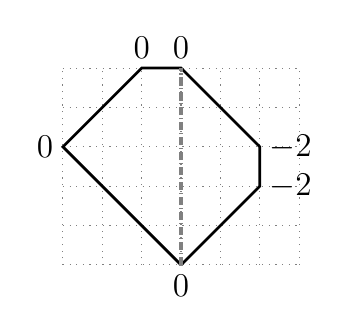
\begin{tikzpicture}[scale=0.5]
   	 \draw[dotted,step=1,gray,] (-3,-3) grid (3,2); \draw[line width = 1pt] (0,-3) --
     (-3,0) -- (-1,2)--(0,2)--
 	 (2,0)--(2,-1) -- (0,-3); \draw[densely dashdotted, gray, line width = 1.2pt] (0,-3) -- (0,2);
 	 \node at (0,-3) [below] {\large{$0$}};
 	 \node at (-3,0) [left] {\large{$0$}};
 	 \node at (-1,2) [above] {\large{$0$}};
 	 \node at (0,2) [above] {\large{$0$}};
 	 \node at (2,0) [right] {\large{$-2$}};
 	 \node at (2,-1) [right] {\large{$-2$}};
	\end{tikzpicture}
	\caption*{$\Phi_0$}
\end{subfigure}
\begin{subfigure}[b]{0.30\textwidth}
	\centering
 	 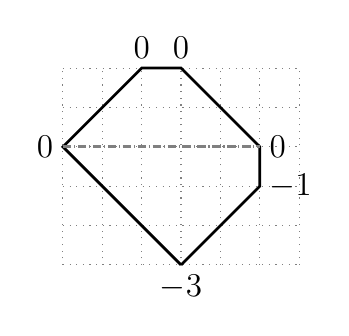
\begin{tikzpicture}[scale=0.5]
 	   \draw[dotted,step=1,gray] (-3,-3) grid (3,2); \draw[line width = 1pt] (0,-3) --
     (-3,0) -- (-1,2)--(0,2)--
 	 (2,0)--(2,-1) -- (0,-3); \draw[densely dashdotted, gray,line width = 1.2pt] (-3,0) -- (2,0);
 	 \node at (0,-3) [below] {\large{$-3$}};
 	 \node at (-3,0) [left] {\large{$0$}};
 	 \node at (-1,2) [above] {\large{$0$}};
 	 \node at (0,2) [above] {\large{$0$}};
 	 \node at (2,0) [right] {\large{$0$}};
 	 \node at (2,-1) [right] {\large{$-1$}};
	\end{tikzpicture}
	\caption*{$\Phi_1$}
\end{subfigure}
\begin{subfigure}[b]{0.30\textwidth}
	\centering
 	 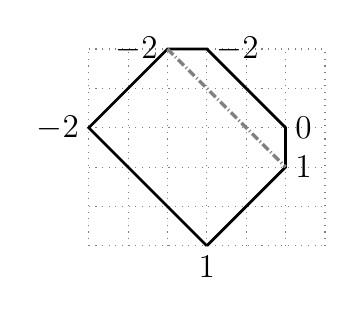
\begin{tikzpicture}[scale=0.5]
 	   \draw[dotted,step=1,gray] (-3,-3) grid (3,2); \draw[line width = 1pt] (0,-3) --
     (-3,0) -- (-1,2)--(0,2)--
 	 (2,0)--(2,-1) -- (0,-3); \draw[densely dashdotted, gray,line width = 1.2pt] (-1,2) -- (2,-1);
 	 \node at (0,-3) [below] {\large{$1$}};
 	 \node at (-3,0) [left] {\large{$-2$}};
 	 \node at (-1,2) [left] {\large{$-2$}};
 	 \node at (0,2) [right] {\large{$-2$}};
 	 \node at (2,0) [right] {\large{$0$}};
 	 \node at (2,-1) [right] {\large{$1$}};
	\end{tikzpicture}
	\caption*{$\Phi_\infty$}
\end{subfigure}
\begin{subfigure}[b]{0.40\textwidth}
	\centering
 	 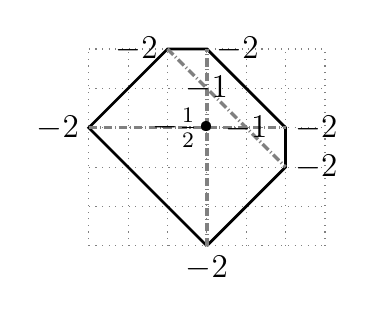
\begin{tikzpicture}[scale=0.5]
 	   \draw[dotted,step=1,gray] (-3,-3) grid (3,2); \draw[line width = 1pt] (0,-3) --
     (-3,0) -- (-1,2)--(0,2)--
 	 (2,0)--(2,-1) -- (0,-3); \draw[densely dashdotted, gray, line width = 1.2pt] (0,-3) -- (0,2);  \draw[densely dashdotted, gray,line width = 1.2pt] (-3,0) -- (2,0); \draw[densely dashdotted, gray,line width = 1.2pt] (-1,2) -- (2,-1);
 	 \node at (0,-3) [below] {\large{$-2$}};
 	 \node at (-3,0) [left] {\large{$-2$}};
 	 \node at (-1,2) [left] {\large{$-2$}};
 	 \node at (0,2) [right] {\large{$-2$}};
 	 \node at (2,0) [right] {\large{$-2$}};
 	 \node at (2,-1) [right] {\large{$-2$}};
 	 \node at (1,0) {\large{$-1$}};
 	 \node at (0,1) {\large{$-1$}};
 	 \node at (0,0) [left] {\large{$-\frac{1}{2}$}};
 	 \draw (0,0) node {\textbullet};
	\end{tikzpicture}
	\caption*{$\deg \Phi $}
\end{subfigure}
}
\end{figure}
\begin{tabularx}{\textwidth}{|c|c|c}
\toprule
\(y\) & \(\text{Vert}(\Delta_y)\) & \(n_y\) \\
\midrule
\(0\) & \begin{tabular}{l} \((-3,0,1),(-2,1,1),(2,1,-1),\) \\ \hspace{1cm} \((3,0,-2),(0,-3,1),(0,1,1)\) \end{tabular} & \((a,b,c)\) \\ \midrule
\(1\) & \begin{tabular}{l} \((-3,0,1),(-2,1,1),(0,1,0),\) \\ \hspace{1cm} \((2,1,1),(3,0,1),(0,-3,-2)\) \end{tabular} & \((a,b,c)\) \\ \midrule
\(\infty\) & \begin{tabular}{l} \((-3,0,-1),(-2,1,-1),(2,1,1),\) \\ \hspace{1cm} \((3,0,2),(0,-3,2),(0,0,-1),(0,1,-1)\) \end{tabular} & \((a,b,c)\) \\
\midrule
\end{tabularx}
\begin{align*}
g(\xi) &= \frac{1}{\xi_{2}^{4}}\cdot\left({\left(2 \, \xi_{2}^{3} - 3 \, \xi_{2} - 3\right)} e^{\left(4 \, \xi_{2}\right)} + 12 \, \xi_{2} e^{\left(3 \, \xi_{2}\right)} + 3 \, \xi_{2} + 3\right) e^{\left(-3 \, \xi_{2}\right)}
\end{align*}
\begin{tabularx}{\textwidth}{|c|c|c}
\toprule
\(y\) & \( h_y(\xi_2)\) & \( h_y(\xi_2) \in\) \\
\midrule
\(0\) & \begin{tabular}{l} \(\frac{1}{3\xi_2^{4}} \cdot
 ( \ (2   \xi_2^{3} - 3   \xi_2 - 3) e^{4   \xi_2} \)   \\ \hspace{2cm} \(+12 \xi_2 e^{3 \xi_2} + 3 \xi_2 + 3 \ ) e^{-3 \xi_2}\) \end{tabular} & \((1.087,1.458)\) \\ \midrule
\(1\) & \begin{tabular}{l} \(\frac{1}{3\xi_2^{4}} \cdot
 ( \ (2   \xi_2^{3} - 3   \xi_2 - 3) e^{4   \xi_2} \)   \\ \hspace{2cm} \(+12 \xi_2 e^{3 \xi_2} + 3 \xi_2 + 3 \ ) e^{-3 \xi_2}\) \end{tabular} & \((2.178,2.470)\) \\ \midrule
\(\infty\) & \begin{tabular}{l} \(\frac{1}{3\xi_2^{4}} \cdot
 ( \ (2   \xi_2^{3} - 3   \xi_2 - 3) e^{4   \xi_2} \)   \\ \hspace{2cm} \(+12 \xi_2 e^{3 \xi_2} + 3 \xi_2 + 3 \ ) e^{-3 \xi_2}\) \end{tabular} & \((0.446,0.827)\) \\ \midrule
\(\notin \{0,1,\infty\}\) & \begin{tabular}{l} \(\frac{1}{3\xi_2^{4}} \cdot
 ( \ (2   \xi_2^{3} - 3   \xi_2 - 3) e^{4   \xi_2} \)   \\ \hspace{2cm} \(+12 \xi_2 e^{3 \xi_2} + 3 \xi_2 + 3 \ ) e^{-3 \xi_2}\) \end{tabular} & \((4.151,4.309)\) \\
 \bottomrule
\end{tabularx}
\newpage
%
%
%
%
%
%
%
%
\begin{tabularx}{\textwidth}{rlrl}
\toprule
\textbf{Name:} & \ 2.31 \hspace{0.3\textwidth} & \textbf{Description:} & Blow up of $Q$ in a line\\
\midrule
\textbf{$\sigma$}: & {\small $\begin{pmatrix} -1 & 0 \\ 0 & 1 \end{pmatrix}$ } & $ R(X) = 23/29$ , & $\xi \sim (0,0.51489)$
\end{tabularx}

\begin{figure}[H]
\centering
\label{fig:data231}
\resizebox{0.9\linewidth}{!}{
\begin{subfigure}[b]{0.30\textwidth}
\centering
  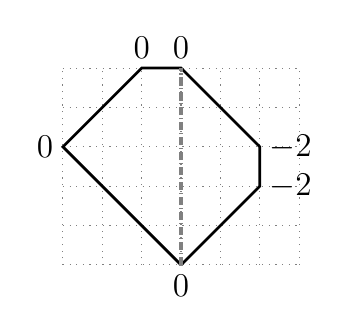
\begin{tikzpicture}[scale=0.5]
   	 \draw[dotted,step=1,gray,] (-3,-3) grid (3,2); \draw[line width = 1pt] (0,-3) --
     (-3,0) -- (-1,2)--(0,2)--
 	 (2,0)--(2,-1) -- (0,-3); \draw[densely dashdotted, gray, line width = 1.2pt] (0,-3) -- (0,2);
 	 \node at (0,-3) [below] {\large{$0$}};
 	 \node at (-3,0) [left] {\large{$0$}};
 	 \node at (-1,2) [above] {\large{$0$}};
 	 \node at (0,2) [above] {\large{$0$}};
 	 \node at (2,0) [right] {\large{$-2$}};
 	 \node at (2,-1) [right] {\large{$-2$}};
	\end{tikzpicture}
	\caption*{$\Phi_0$}
\end{subfigure}
\begin{subfigure}[b]{0.30\textwidth}
	\centering
 	 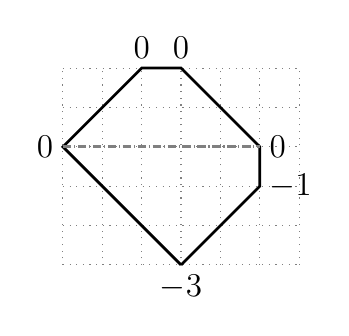
\begin{tikzpicture}[scale=0.5]
 	   \draw[dotted,step=1,gray] (-3,-3) grid (3,2); \draw[line width = 1pt] (0,-3) --
     (-3,0) -- (-1,2)--(0,2)--
 	 (2,0)--(2,-1) -- (0,-3); \draw[densely dashdotted, gray,line width = 1.2pt] (-3,0) -- (2,0);
 	 \node at (0,-3) [below] {\large{$-3$}};
 	 \node at (-3,0) [left] {\large{$0$}};
 	 \node at (-1,2) [above] {\large{$0$}};
 	 \node at (0,2) [above] {\large{$0$}};
 	 \node at (2,0) [right] {\large{$0$}};
 	 \node at (2,-1) [right] {\large{$-1$}};
	\end{tikzpicture}
	\caption*{$\Phi_1$}
\end{subfigure}
\begin{subfigure}[b]{0.30\textwidth}
	\centering
 	 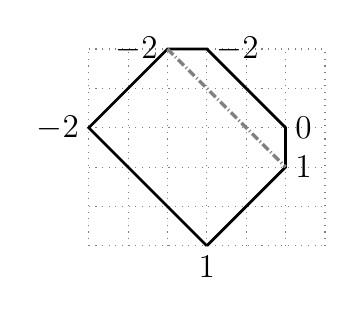
\begin{tikzpicture}[scale=0.5]
 	   \draw[dotted,step=1,gray] (-3,-3) grid (3,2); \draw[line width = 1pt] (0,-3) --
     (-3,0) -- (-1,2)--(0,2)--
 	 (2,0)--(2,-1) -- (0,-3); \draw[densely dashdotted, gray,line width = 1.2pt] (-1,2) -- (2,-1);
 	 \node at (0,-3) [below] {\large{$1$}};
 	 \node at (-3,0) [left] {\large{$-2$}};
 	 \node at (-1,2) [left] {\large{$-2$}};
 	 \node at (0,2) [right] {\large{$-2$}};
 	 \node at (2,0) [right] {\large{$0$}};
 	 \node at (2,-1) [right] {\large{$1$}};
	\end{tikzpicture}
	\caption*{$\Phi_\infty$}
\end{subfigure}
\begin{subfigure}[b]{0.40\textwidth}
	\centering
 	 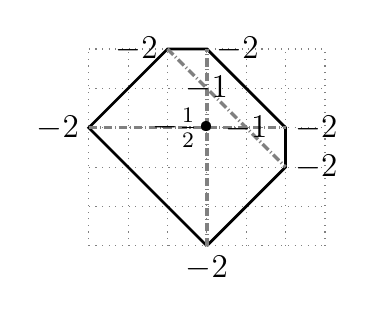
\begin{tikzpicture}[scale=0.5]
 	   \draw[dotted,step=1,gray] (-3,-3) grid (3,2); \draw[line width = 1pt] (0,-3) --
     (-3,0) -- (-1,2)--(0,2)--
 	 (2,0)--(2,-1) -- (0,-3); \draw[densely dashdotted, gray, line width = 1.2pt] (0,-3) -- (0,2);  \draw[densely dashdotted, gray,line width = 1.2pt] (-3,0) -- (2,0); \draw[densely dashdotted, gray,line width = 1.2pt] (-1,2) -- (2,-1);
 	 \node at (0,-3) [below] {\large{$-2$}};
 	 \node at (-3,0) [left] {\large{$-2$}};
 	 \node at (-1,2) [left] {\large{$-2$}};
 	 \node at (0,2) [right] {\large{$-2$}};
 	 \node at (2,0) [right] {\large{$-2$}};
 	 \node at (2,-1) [right] {\large{$-2$}};
 	 \node at (1,0) {\large{$-1$}};
 	 \node at (0,1) {\large{$-1$}};
 	 \node at (0,0) [left] {\large{$-\frac{1}{2}$}};
 	 \draw (0,0) node {\textbullet};
	\end{tikzpicture}
	\caption*{$\deg \Phi $}
\end{subfigure}
}
\end{figure}
\begin{tabularx}{\textwidth}{|c|c|c}
\toprule
\(y\) & \(\text{Vert}(\Delta_y)\) & \(n_y\) \\
\midrule
\(0\) & \begin{tabular}{l} \((-3,0,1),(-2,1,1),(2,1,-1),\) \\ \hspace{1cm} \((3,0,-2),(0,-3,1),(0,1,1)\) \end{tabular} & \((a,b,c)\) \\ \midrule
\(1\) & \begin{tabular}{l} \((-3,0,1),(-2,1,1),(0,1,0),\) \\ \hspace{1cm} \((2,1,1),(3,0,1),(0,-3,-2)\) \end{tabular} & \((a,b,c)\) \\ \midrule
\(\infty\) & \begin{tabular}{l} \((-3,0,-1),(-2,1,-1),(2,1,1),\) \\ \hspace{1cm} \((3,0,2),(0,-3,2),(0,0,-1),(0,1,-1)\) \end{tabular} & \((a,b,c)\) \\
\midrule
\end{tabularx}
\begin{align*}
g(\xi) &= \frac{1}{\xi_{2}^{4}}\cdot\left({\left(2 \, \xi_{2}^{3} - 3 \, \xi_{2} - 3\right)} e^{\left(4 \, \xi_{2}\right)} + 12 \, \xi_{2} e^{\left(3 \, \xi_{2}\right)} + 3 \, \xi_{2} + 3\right) e^{\left(-3 \, \xi_{2}\right)}
\end{align*}
\begin{tabularx}{\textwidth}{|c|c|c}
\toprule
\(y\) & \( h_y(\xi_2)\) & \( h_y(\xi_2) \in\) \\
\midrule
\(0\) & \begin{tabular}{l} \(\frac{1}{3\xi_2^{4}} \cdot
 ( \ (2   \xi_2^{3} - 3   \xi_2 - 3) e^{4   \xi_2} \)   \\ \hspace{2cm} \(+12 \xi_2 e^{3 \xi_2} + 3 \xi_2 + 3 \ ) e^{-3 \xi_2}\) \end{tabular} & \((1.087,1.458)\) \\ \midrule
\(1\) & \begin{tabular}{l} \(\frac{1}{3\xi_2^{4}} \cdot
 ( \ (2   \xi_2^{3} - 3   \xi_2 - 3) e^{4   \xi_2} \)   \\ \hspace{2cm} \(+12 \xi_2 e^{3 \xi_2} + 3 \xi_2 + 3 \ ) e^{-3 \xi_2}\) \end{tabular} & \((2.178,2.470)\) \\ \midrule
\(\infty\) & \begin{tabular}{l} \(\frac{1}{3\xi_2^{4}} \cdot
 ( \ (2   \xi_2^{3} - 3   \xi_2 - 3) e^{4   \xi_2} \)   \\ \hspace{2cm} \(+12 \xi_2 e^{3 \xi_2} + 3 \xi_2 + 3 \ ) e^{-3 \xi_2}\) \end{tabular} & \((0.446,0.827)\) \\ \midrule
\(\notin \{0,1,\infty\}\) & \begin{tabular}{l} \(\frac{1}{3\xi_2^{4}} \cdot
 ( \ (2   \xi_2^{3} - 3   \xi_2 - 3) e^{4   \xi_2} \)   \\ \hspace{2cm} \(+12 \xi_2 e^{3 \xi_2} + 3 \xi_2 + 3 \ ) e^{-3 \xi_2}\) \end{tabular} & \((4.151,4.309)\) \\
 \bottomrule
\end{tabularx}
\newpage
%
%
%
%
%
%
%
%
\begin{tabularx}{\textwidth}{rlrl}
\toprule
\textbf{Name:} & \ 2.31 \hspace{0.3\textwidth} & \textbf{Description:} & Blow up of $Q$ in a line\\
\midrule
\textbf{$\sigma$}: & {\small $\begin{pmatrix} -1 & 0 \\ 0 & 1 \end{pmatrix}$ } & $ R(X) = 23/29$ , & $\xi \sim (0,0.51489)$
\end{tabularx}

\begin{figure}[H]
\centering
\label{fig:data231}
\resizebox{0.9\linewidth}{!}{
\begin{subfigure}[b]{0.30\textwidth}
\centering
  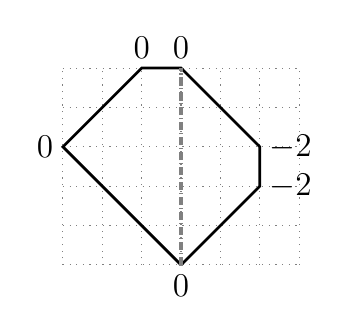
\begin{tikzpicture}[scale=0.5]
   	 \draw[dotted,step=1,gray,] (-3,-3) grid (3,2); \draw[line width = 1pt] (0,-3) --
     (-3,0) -- (-1,2)--(0,2)--
 	 (2,0)--(2,-1) -- (0,-3); \draw[densely dashdotted, gray, line width = 1.2pt] (0,-3) -- (0,2);
 	 \node at (0,-3) [below] {\large{$0$}};
 	 \node at (-3,0) [left] {\large{$0$}};
 	 \node at (-1,2) [above] {\large{$0$}};
 	 \node at (0,2) [above] {\large{$0$}};
 	 \node at (2,0) [right] {\large{$-2$}};
 	 \node at (2,-1) [right] {\large{$-2$}};
	\end{tikzpicture}
	\caption*{$\Phi_0$}
\end{subfigure}
\begin{subfigure}[b]{0.30\textwidth}
	\centering
 	 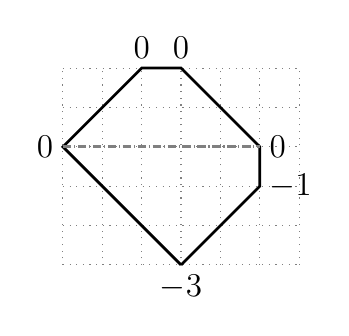
\begin{tikzpicture}[scale=0.5]
 	   \draw[dotted,step=1,gray] (-3,-3) grid (3,2); \draw[line width = 1pt] (0,-3) --
     (-3,0) -- (-1,2)--(0,2)--
 	 (2,0)--(2,-1) -- (0,-3); \draw[densely dashdotted, gray,line width = 1.2pt] (-3,0) -- (2,0);
 	 \node at (0,-3) [below] {\large{$-3$}};
 	 \node at (-3,0) [left] {\large{$0$}};
 	 \node at (-1,2) [above] {\large{$0$}};
 	 \node at (0,2) [above] {\large{$0$}};
 	 \node at (2,0) [right] {\large{$0$}};
 	 \node at (2,-1) [right] {\large{$-1$}};
	\end{tikzpicture}
	\caption*{$\Phi_1$}
\end{subfigure}
\begin{subfigure}[b]{0.30\textwidth}
	\centering
 	 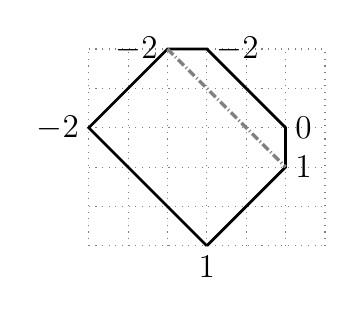
\begin{tikzpicture}[scale=0.5]
 	   \draw[dotted,step=1,gray] (-3,-3) grid (3,2); \draw[line width = 1pt] (0,-3) --
     (-3,0) -- (-1,2)--(0,2)--
 	 (2,0)--(2,-1) -- (0,-3); \draw[densely dashdotted, gray,line width = 1.2pt] (-1,2) -- (2,-1);
 	 \node at (0,-3) [below] {\large{$1$}};
 	 \node at (-3,0) [left] {\large{$-2$}};
 	 \node at (-1,2) [left] {\large{$-2$}};
 	 \node at (0,2) [right] {\large{$-2$}};
 	 \node at (2,0) [right] {\large{$0$}};
 	 \node at (2,-1) [right] {\large{$1$}};
	\end{tikzpicture}
	\caption*{$\Phi_\infty$}
\end{subfigure}
\begin{subfigure}[b]{0.40\textwidth}
	\centering
 	 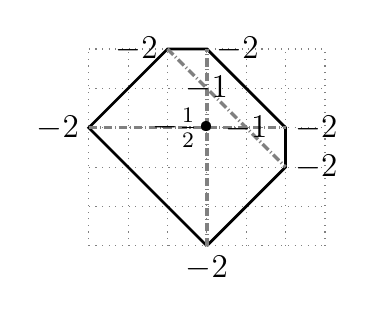
\begin{tikzpicture}[scale=0.5]
 	   \draw[dotted,step=1,gray] (-3,-3) grid (3,2); \draw[line width = 1pt] (0,-3) --
     (-3,0) -- (-1,2)--(0,2)--
 	 (2,0)--(2,-1) -- (0,-3); \draw[densely dashdotted, gray, line width = 1.2pt] (0,-3) -- (0,2);  \draw[densely dashdotted, gray,line width = 1.2pt] (-3,0) -- (2,0); \draw[densely dashdotted, gray,line width = 1.2pt] (-1,2) -- (2,-1);
 	 \node at (0,-3) [below] {\large{$-2$}};
 	 \node at (-3,0) [left] {\large{$-2$}};
 	 \node at (-1,2) [left] {\large{$-2$}};
 	 \node at (0,2) [right] {\large{$-2$}};
 	 \node at (2,0) [right] {\large{$-2$}};
 	 \node at (2,-1) [right] {\large{$-2$}};
 	 \node at (1,0) {\large{$-1$}};
 	 \node at (0,1) {\large{$-1$}};
 	 \node at (0,0) [left] {\large{$-\frac{1}{2}$}};
 	 \draw (0,0) node {\textbullet};
	\end{tikzpicture}
	\caption*{$\deg \Phi $}
\end{subfigure}
}
\end{figure}
\begin{tabularx}{\textwidth}{|c|c|c}
\toprule
\(y\) & \(\text{Vert}(\Delta_y)\) & \(n_y\) \\
\midrule
\(0\) & \begin{tabular}{l} \((-3,0,1),(-2,1,1),(2,1,-1),\) \\ \hspace{1cm} \((3,0,-2),(0,-3,1),(0,1,1)\) \end{tabular} & \((a,b,c)\) \\ \midrule
\(1\) & \begin{tabular}{l} \((-3,0,1),(-2,1,1),(0,1,0),\) \\ \hspace{1cm} \((2,1,1),(3,0,1),(0,-3,-2)\) \end{tabular} & \((a,b,c)\) \\ \midrule
\(\infty\) & \begin{tabular}{l} \((-3,0,-1),(-2,1,-1),(2,1,1),\) \\ \hspace{1cm} \((3,0,2),(0,-3,2),(0,0,-1),(0,1,-1)\) \end{tabular} & \((a,b,c)\) \\
\midrule
\end{tabularx}
\begin{align*}
g(\xi) &= \frac{1}{\xi_{2}^{4}}\cdot\left({\left(2 \, \xi_{2}^{3} - 3 \, \xi_{2} - 3\right)} e^{\left(4 \, \xi_{2}\right)} + 12 \, \xi_{2} e^{\left(3 \, \xi_{2}\right)} + 3 \, \xi_{2} + 3\right) e^{\left(-3 \, \xi_{2}\right)}
\end{align*}
\begin{tabularx}{\textwidth}{|c|c|c}
\toprule
\(y\) & \( h_y(\xi_2)\) & \( h_y(\xi_2) \in\) \\
\midrule
\(0\) & \begin{tabular}{l} \(\frac{1}{3\xi_2^{4}} \cdot
 ( \ (2   \xi_2^{3} - 3   \xi_2 - 3) e^{4   \xi_2} \)   \\ \hspace{2cm} \(+12 \xi_2 e^{3 \xi_2} + 3 \xi_2 + 3 \ ) e^{-3 \xi_2}\) \end{tabular} & \((1.087,1.458)\) \\ \midrule
\(1\) & \begin{tabular}{l} \(\frac{1}{3\xi_2^{4}} \cdot
 ( \ (2   \xi_2^{3} - 3   \xi_2 - 3) e^{4   \xi_2} \)   \\ \hspace{2cm} \(+12 \xi_2 e^{3 \xi_2} + 3 \xi_2 + 3 \ ) e^{-3 \xi_2}\) \end{tabular} & \((2.178,2.470)\) \\ \midrule
\(\infty\) & \begin{tabular}{l} \(\frac{1}{3\xi_2^{4}} \cdot
 ( \ (2   \xi_2^{3} - 3   \xi_2 - 3) e^{4   \xi_2} \)   \\ \hspace{2cm} \(+12 \xi_2 e^{3 \xi_2} + 3 \xi_2 + 3 \ ) e^{-3 \xi_2}\) \end{tabular} & \((0.446,0.827)\) \\ \midrule
\(\notin \{0,1,\infty\}\) & \begin{tabular}{l} \(\frac{1}{3\xi_2^{4}} \cdot
 ( \ (2   \xi_2^{3} - 3   \xi_2 - 3) e^{4   \xi_2} \)   \\ \hspace{2cm} \(+12 \xi_2 e^{3 \xi_2} + 3 \xi_2 + 3 \ ) e^{-3 \xi_2}\) \end{tabular} & \((4.151,4.309)\) \\
 \bottomrule
\end{tabularx}
\newpage
%
%
%
%
%
%
%
%
\begin{tabularx}{\textwidth}{rlrl}
\toprule
\textbf{Name:} & \ 2.31 \hspace{0.3\textwidth} & \textbf{Description:} & Blow up of $Q$ in a line\\
\midrule
\textbf{$\sigma$}: & {\small $\begin{pmatrix} -1 & 0 \\ 0 & 1 \end{pmatrix}$ } & $ R(X) = 23/29$ , & $\xi \sim (0,0.51489)$
\end{tabularx}

\begin{figure}[H]
\centering
\label{fig:data231}
\resizebox{0.9\linewidth}{!}{
\begin{subfigure}[b]{0.30\textwidth}
\centering
  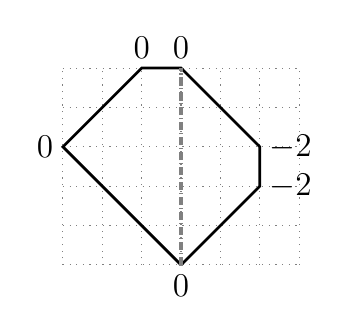
\begin{tikzpicture}[scale=0.5]
   	 \draw[dotted,step=1,gray,] (-3,-3) grid (3,2); \draw[line width = 1pt] (0,-3) --
     (-3,0) -- (-1,2)--(0,2)--
 	 (2,0)--(2,-1) -- (0,-3); \draw[densely dashdotted, gray, line width = 1.2pt] (0,-3) -- (0,2);
 	 \node at (0,-3) [below] {\large{$0$}};
 	 \node at (-3,0) [left] {\large{$0$}};
 	 \node at (-1,2) [above] {\large{$0$}};
 	 \node at (0,2) [above] {\large{$0$}};
 	 \node at (2,0) [right] {\large{$-2$}};
 	 \node at (2,-1) [right] {\large{$-2$}};
	\end{tikzpicture}
	\caption*{$\Phi_0$}
\end{subfigure}
\begin{subfigure}[b]{0.30\textwidth}
	\centering
 	 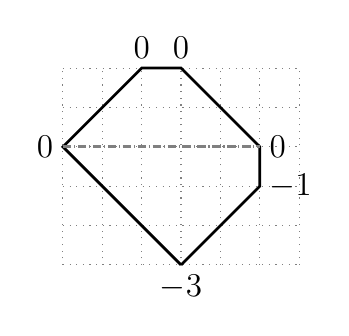
\begin{tikzpicture}[scale=0.5]
 	   \draw[dotted,step=1,gray] (-3,-3) grid (3,2); \draw[line width = 1pt] (0,-3) --
     (-3,0) -- (-1,2)--(0,2)--
 	 (2,0)--(2,-1) -- (0,-3); \draw[densely dashdotted, gray,line width = 1.2pt] (-3,0) -- (2,0);
 	 \node at (0,-3) [below] {\large{$-3$}};
 	 \node at (-3,0) [left] {\large{$0$}};
 	 \node at (-1,2) [above] {\large{$0$}};
 	 \node at (0,2) [above] {\large{$0$}};
 	 \node at (2,0) [right] {\large{$0$}};
 	 \node at (2,-1) [right] {\large{$-1$}};
	\end{tikzpicture}
	\caption*{$\Phi_1$}
\end{subfigure}
\begin{subfigure}[b]{0.30\textwidth}
	\centering
 	 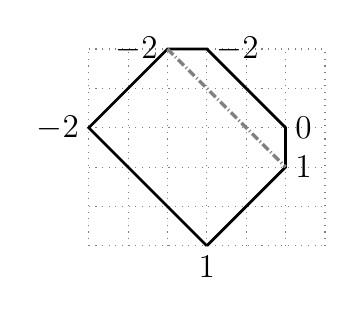
\begin{tikzpicture}[scale=0.5]
 	   \draw[dotted,step=1,gray] (-3,-3) grid (3,2); \draw[line width = 1pt] (0,-3) --
     (-3,0) -- (-1,2)--(0,2)--
 	 (2,0)--(2,-1) -- (0,-3); \draw[densely dashdotted, gray,line width = 1.2pt] (-1,2) -- (2,-1);
 	 \node at (0,-3) [below] {\large{$1$}};
 	 \node at (-3,0) [left] {\large{$-2$}};
 	 \node at (-1,2) [left] {\large{$-2$}};
 	 \node at (0,2) [right] {\large{$-2$}};
 	 \node at (2,0) [right] {\large{$0$}};
 	 \node at (2,-1) [right] {\large{$1$}};
	\end{tikzpicture}
	\caption*{$\Phi_\infty$}
\end{subfigure}
\begin{subfigure}[b]{0.40\textwidth}
	\centering
 	 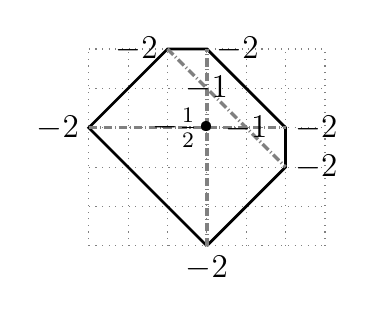
\begin{tikzpicture}[scale=0.5]
 	   \draw[dotted,step=1,gray] (-3,-3) grid (3,2); \draw[line width = 1pt] (0,-3) --
     (-3,0) -- (-1,2)--(0,2)--
 	 (2,0)--(2,-1) -- (0,-3); \draw[densely dashdotted, gray, line width = 1.2pt] (0,-3) -- (0,2);  \draw[densely dashdotted, gray,line width = 1.2pt] (-3,0) -- (2,0); \draw[densely dashdotted, gray,line width = 1.2pt] (-1,2) -- (2,-1);
 	 \node at (0,-3) [below] {\large{$-2$}};
 	 \node at (-3,0) [left] {\large{$-2$}};
 	 \node at (-1,2) [left] {\large{$-2$}};
 	 \node at (0,2) [right] {\large{$-2$}};
 	 \node at (2,0) [right] {\large{$-2$}};
 	 \node at (2,-1) [right] {\large{$-2$}};
 	 \node at (1,0) {\large{$-1$}};
 	 \node at (0,1) {\large{$-1$}};
 	 \node at (0,0) [left] {\large{$-\frac{1}{2}$}};
 	 \draw (0,0) node {\textbullet};
	\end{tikzpicture}
	\caption*{$\deg \Phi $}
\end{subfigure}
}
\end{figure}
\begin{tabularx}{\textwidth}{|c|c|c}
\toprule
\(y\) & \(\text{Vert}(\Delta_y)\) & \(n_y\) \\
\midrule
\(0\) & \begin{tabular}{l} \((-3,0,1),(-2,1,1),(2,1,-1),\) \\ \hspace{1cm} \((3,0,-2),(0,-3,1),(0,1,1)\) \end{tabular} & \((a,b,c)\) \\ \midrule
\(1\) & \begin{tabular}{l} \((-3,0,1),(-2,1,1),(0,1,0),\) \\ \hspace{1cm} \((2,1,1),(3,0,1),(0,-3,-2)\) \end{tabular} & \((a,b,c)\) \\ \midrule
\(\infty\) & \begin{tabular}{l} \((-3,0,-1),(-2,1,-1),(2,1,1),\) \\ \hspace{1cm} \((3,0,2),(0,-3,2),(0,0,-1),(0,1,-1)\) \end{tabular} & \((a,b,c)\) \\
\midrule
\end{tabularx}
\begin{align*}
g(\xi) &= \frac{1}{\xi_{2}^{4}}\cdot\left({\left(2 \, \xi_{2}^{3} - 3 \, \xi_{2} - 3\right)} e^{\left(4 \, \xi_{2}\right)} + 12 \, \xi_{2} e^{\left(3 \, \xi_{2}\right)} + 3 \, \xi_{2} + 3\right) e^{\left(-3 \, \xi_{2}\right)}
\end{align*}
\begin{tabularx}{\textwidth}{|c|c|c}
\toprule
\(y\) & \( h_y(\xi_2)\) & \( h_y(\xi_2) \in\) \\
\midrule
\(0\) & \begin{tabular}{l} \(\frac{1}{3\xi_2^{4}} \cdot
 ( \ (2   \xi_2^{3} - 3   \xi_2 - 3) e^{4   \xi_2} \)   \\ \hspace{2cm} \(+12 \xi_2 e^{3 \xi_2} + 3 \xi_2 + 3 \ ) e^{-3 \xi_2}\) \end{tabular} & \((1.087,1.458)\) \\ \midrule
\(1\) & \begin{tabular}{l} \(\frac{1}{3\xi_2^{4}} \cdot
 ( \ (2   \xi_2^{3} - 3   \xi_2 - 3) e^{4   \xi_2} \)   \\ \hspace{2cm} \(+12 \xi_2 e^{3 \xi_2} + 3 \xi_2 + 3 \ ) e^{-3 \xi_2}\) \end{tabular} & \((2.178,2.470)\) \\ \midrule
\(\infty\) & \begin{tabular}{l} \(\frac{1}{3\xi_2^{4}} \cdot
 ( \ (2   \xi_2^{3} - 3   \xi_2 - 3) e^{4   \xi_2} \)   \\ \hspace{2cm} \(+12 \xi_2 e^{3 \xi_2} + 3 \xi_2 + 3 \ ) e^{-3 \xi_2}\) \end{tabular} & \((0.446,0.827)\) \\ \midrule
\(\notin \{0,1,\infty\}\) & \begin{tabular}{l} \(\frac{1}{3\xi_2^{4}} \cdot
 ( \ (2   \xi_2^{3} - 3   \xi_2 - 3) e^{4   \xi_2} \)   \\ \hspace{2cm} \(+12 \xi_2 e^{3 \xi_2} + 3 \xi_2 + 3 \ ) e^{-3 \xi_2}\) \end{tabular} & \((4.151,4.309)\) \\
 \bottomrule
\end{tabularx}
\newpage
%
%
%
%
%
%
%
%
\begin{tabularx}{\textwidth}{rlrl}
\toprule
\textbf{Name:} & \ 2.31 \hspace{0.3\textwidth} & \textbf{Description:} & Blow up of $Q$ in a line\\
\midrule
\textbf{$\sigma$}: & {\small $\begin{pmatrix} -1 & 0 \\ 0 & 1 \end{pmatrix}$ } & $ R(X) = 23/29$ , & $\xi \sim (0,0.51489)$
\end{tabularx}

\begin{figure}[H]
\centering
\label{fig:data231}
\resizebox{0.9\linewidth}{!}{
\begin{subfigure}[b]{0.30\textwidth}
\centering
  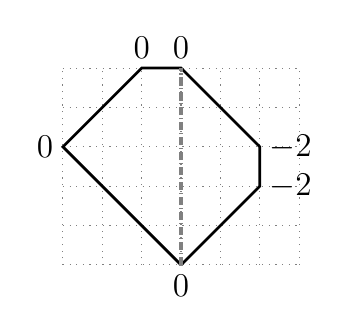
\begin{tikzpicture}[scale=0.5]
   	 \draw[dotted,step=1,gray,] (-3,-3) grid (3,2); \draw[line width = 1pt] (0,-3) --
     (-3,0) -- (-1,2)--(0,2)--
 	 (2,0)--(2,-1) -- (0,-3); \draw[densely dashdotted, gray, line width = 1.2pt] (0,-3) -- (0,2);
 	 \node at (0,-3) [below] {\large{$0$}};
 	 \node at (-3,0) [left] {\large{$0$}};
 	 \node at (-1,2) [above] {\large{$0$}};
 	 \node at (0,2) [above] {\large{$0$}};
 	 \node at (2,0) [right] {\large{$-2$}};
 	 \node at (2,-1) [right] {\large{$-2$}};
	\end{tikzpicture}
	\caption*{$\Phi_0$}
\end{subfigure}
\begin{subfigure}[b]{0.30\textwidth}
	\centering
 	 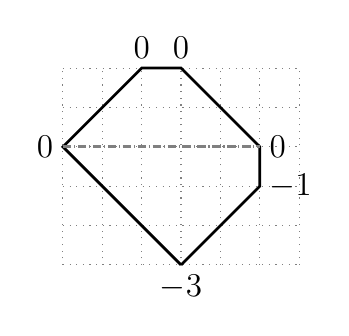
\begin{tikzpicture}[scale=0.5]
 	   \draw[dotted,step=1,gray] (-3,-3) grid (3,2); \draw[line width = 1pt] (0,-3) --
     (-3,0) -- (-1,2)--(0,2)--
 	 (2,0)--(2,-1) -- (0,-3); \draw[densely dashdotted, gray,line width = 1.2pt] (-3,0) -- (2,0);
 	 \node at (0,-3) [below] {\large{$-3$}};
 	 \node at (-3,0) [left] {\large{$0$}};
 	 \node at (-1,2) [above] {\large{$0$}};
 	 \node at (0,2) [above] {\large{$0$}};
 	 \node at (2,0) [right] {\large{$0$}};
 	 \node at (2,-1) [right] {\large{$-1$}};
	\end{tikzpicture}
	\caption*{$\Phi_1$}
\end{subfigure}
\begin{subfigure}[b]{0.30\textwidth}
	\centering
 	 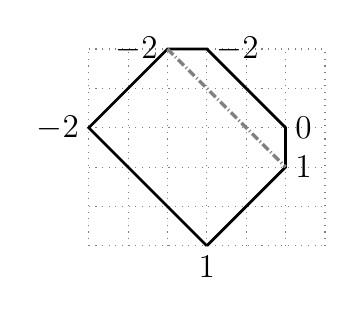
\begin{tikzpicture}[scale=0.5]
 	   \draw[dotted,step=1,gray] (-3,-3) grid (3,2); \draw[line width = 1pt] (0,-3) --
     (-3,0) -- (-1,2)--(0,2)--
 	 (2,0)--(2,-1) -- (0,-3); \draw[densely dashdotted, gray,line width = 1.2pt] (-1,2) -- (2,-1);
 	 \node at (0,-3) [below] {\large{$1$}};
 	 \node at (-3,0) [left] {\large{$-2$}};
 	 \node at (-1,2) [left] {\large{$-2$}};
 	 \node at (0,2) [right] {\large{$-2$}};
 	 \node at (2,0) [right] {\large{$0$}};
 	 \node at (2,-1) [right] {\large{$1$}};
	\end{tikzpicture}
	\caption*{$\Phi_\infty$}
\end{subfigure}
\begin{subfigure}[b]{0.40\textwidth}
	\centering
 	 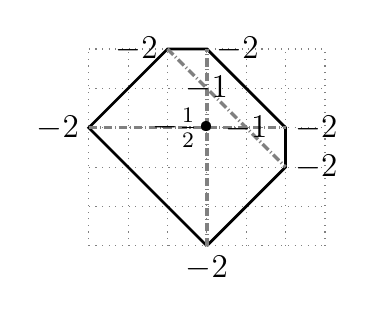
\begin{tikzpicture}[scale=0.5]
 	   \draw[dotted,step=1,gray] (-3,-3) grid (3,2); \draw[line width = 1pt] (0,-3) --
     (-3,0) -- (-1,2)--(0,2)--
 	 (2,0)--(2,-1) -- (0,-3); \draw[densely dashdotted, gray, line width = 1.2pt] (0,-3) -- (0,2);  \draw[densely dashdotted, gray,line width = 1.2pt] (-3,0) -- (2,0); \draw[densely dashdotted, gray,line width = 1.2pt] (-1,2) -- (2,-1);
 	 \node at (0,-3) [below] {\large{$-2$}};
 	 \node at (-3,0) [left] {\large{$-2$}};
 	 \node at (-1,2) [left] {\large{$-2$}};
 	 \node at (0,2) [right] {\large{$-2$}};
 	 \node at (2,0) [right] {\large{$-2$}};
 	 \node at (2,-1) [right] {\large{$-2$}};
 	 \node at (1,0) {\large{$-1$}};
 	 \node at (0,1) {\large{$-1$}};
 	 \node at (0,0) [left] {\large{$-\frac{1}{2}$}};
 	 \draw (0,0) node {\textbullet};
	\end{tikzpicture}
	\caption*{$\deg \Phi $}
\end{subfigure}
}
\end{figure}
\begin{tabularx}{\textwidth}{|c|c|c}
\toprule
\(y\) & \(\text{Vert}(\Delta_y)\) & \(n_y\) \\
\midrule
\(0\) & \begin{tabular}{l} \((-3,0,1),(-2,1,1),(2,1,-1),\) \\ \hspace{1cm} \((3,0,-2),(0,-3,1),(0,1,1)\) \end{tabular} & \((a,b,c)\) \\ \midrule
\(1\) & \begin{tabular}{l} \((-3,0,1),(-2,1,1),(0,1,0),\) \\ \hspace{1cm} \((2,1,1),(3,0,1),(0,-3,-2)\) \end{tabular} & \((a,b,c)\) \\ \midrule
\(\infty\) & \begin{tabular}{l} \((-3,0,-1),(-2,1,-1),(2,1,1),\) \\ \hspace{1cm} \((3,0,2),(0,-3,2),(0,0,-1),(0,1,-1)\) \end{tabular} & \((a,b,c)\) \\
\midrule
\end{tabularx}
\begin{align*}
g(\xi) &= \frac{1}{\xi_{2}^{4}}\cdot\left({\left(2 \, \xi_{2}^{3} - 3 \, \xi_{2} - 3\right)} e^{\left(4 \, \xi_{2}\right)} + 12 \, \xi_{2} e^{\left(3 \, \xi_{2}\right)} + 3 \, \xi_{2} + 3\right) e^{\left(-3 \, \xi_{2}\right)}
\end{align*}
\begin{tabularx}{\textwidth}{|c|c|c}
\toprule
\(y\) & \( h_y(\xi_2)\) & \( h_y(\xi_2) \in\) \\
\midrule
\(0\) & \begin{tabular}{l} \(\frac{1}{3\xi_2^{4}} \cdot
 ( \ (2   \xi_2^{3} - 3   \xi_2 - 3) e^{4   \xi_2} \)   \\ \hspace{2cm} \(+12 \xi_2 e^{3 \xi_2} + 3 \xi_2 + 3 \ ) e^{-3 \xi_2}\) \end{tabular} & \((1.087,1.458)\) \\ \midrule
\(1\) & \begin{tabular}{l} \(\frac{1}{3\xi_2^{4}} \cdot
 ( \ (2   \xi_2^{3} - 3   \xi_2 - 3) e^{4   \xi_2} \)   \\ \hspace{2cm} \(+12 \xi_2 e^{3 \xi_2} + 3 \xi_2 + 3 \ ) e^{-3 \xi_2}\) \end{tabular} & \((2.178,2.470)\) \\ \midrule
\(\infty\) & \begin{tabular}{l} \(\frac{1}{3\xi_2^{4}} \cdot
 ( \ (2   \xi_2^{3} - 3   \xi_2 - 3) e^{4   \xi_2} \)   \\ \hspace{2cm} \(+12 \xi_2 e^{3 \xi_2} + 3 \xi_2 + 3 \ ) e^{-3 \xi_2}\) \end{tabular} & \((0.446,0.827)\) \\ \midrule
\(\notin \{0,1,\infty\}\) & \begin{tabular}{l} \(\frac{1}{3\xi_2^{4}} \cdot
 ( \ (2   \xi_2^{3} - 3   \xi_2 - 3) e^{4   \xi_2} \)   \\ \hspace{2cm} \(+12 \xi_2 e^{3 \xi_2} + 3 \xi_2 + 3 \ ) e^{-3 \xi_2}\) \end{tabular} & \((4.151,4.309)\) \\
 \bottomrule
\end{tabularx}
\newpage
%
%
%
%
%
%
%
%
\begin{tabularx}{\textwidth}{rlrl}
\toprule
\textbf{Name:} & \ 2.31 \hspace{0.3\textwidth} & \textbf{Description:} & Blow up of $Q$ in a line\\
\midrule
\textbf{$\sigma$}: & {\small $\begin{pmatrix} -1 & 0 \\ 0 & 1 \end{pmatrix}$ } & $ R(X) = 23/29$ , & $\xi \sim (0,0.51489)$
\end{tabularx}

\begin{figure}[H]
\centering
\label{fig:data231}
\resizebox{0.9\linewidth}{!}{
\begin{subfigure}[b]{0.30\textwidth}
\centering
  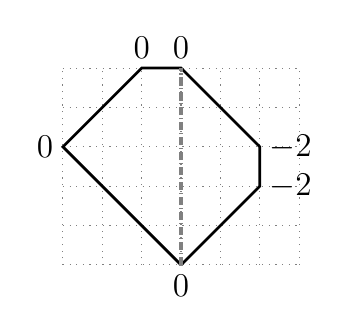
\begin{tikzpicture}[scale=0.5]
   	 \draw[dotted,step=1,gray,] (-3,-3) grid (3,2); \draw[line width = 1pt] (0,-3) --
     (-3,0) -- (-1,2)--(0,2)--
 	 (2,0)--(2,-1) -- (0,-3); \draw[densely dashdotted, gray, line width = 1.2pt] (0,-3) -- (0,2);
 	 \node at (0,-3) [below] {\large{$0$}};
 	 \node at (-3,0) [left] {\large{$0$}};
 	 \node at (-1,2) [above] {\large{$0$}};
 	 \node at (0,2) [above] {\large{$0$}};
 	 \node at (2,0) [right] {\large{$-2$}};
 	 \node at (2,-1) [right] {\large{$-2$}};
	\end{tikzpicture}
	\caption*{$\Phi_0$}
\end{subfigure}
\begin{subfigure}[b]{0.30\textwidth}
	\centering
 	 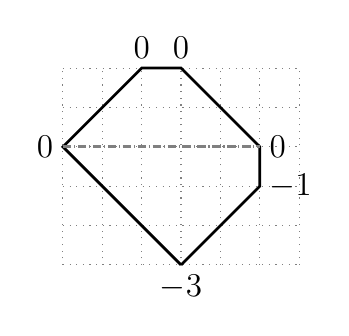
\begin{tikzpicture}[scale=0.5]
 	   \draw[dotted,step=1,gray] (-3,-3) grid (3,2); \draw[line width = 1pt] (0,-3) --
     (-3,0) -- (-1,2)--(0,2)--
 	 (2,0)--(2,-1) -- (0,-3); \draw[densely dashdotted, gray,line width = 1.2pt] (-3,0) -- (2,0);
 	 \node at (0,-3) [below] {\large{$-3$}};
 	 \node at (-3,0) [left] {\large{$0$}};
 	 \node at (-1,2) [above] {\large{$0$}};
 	 \node at (0,2) [above] {\large{$0$}};
 	 \node at (2,0) [right] {\large{$0$}};
 	 \node at (2,-1) [right] {\large{$-1$}};
	\end{tikzpicture}
	\caption*{$\Phi_1$}
\end{subfigure}
\begin{subfigure}[b]{0.30\textwidth}
	\centering
 	 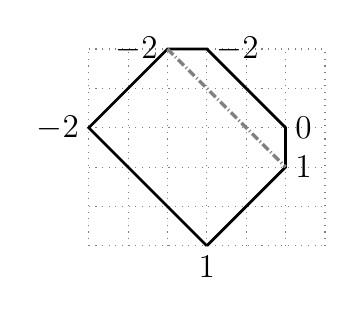
\begin{tikzpicture}[scale=0.5]
 	   \draw[dotted,step=1,gray] (-3,-3) grid (3,2); \draw[line width = 1pt] (0,-3) --
     (-3,0) -- (-1,2)--(0,2)--
 	 (2,0)--(2,-1) -- (0,-3); \draw[densely dashdotted, gray,line width = 1.2pt] (-1,2) -- (2,-1);
 	 \node at (0,-3) [below] {\large{$1$}};
 	 \node at (-3,0) [left] {\large{$-2$}};
 	 \node at (-1,2) [left] {\large{$-2$}};
 	 \node at (0,2) [right] {\large{$-2$}};
 	 \node at (2,0) [right] {\large{$0$}};
 	 \node at (2,-1) [right] {\large{$1$}};
	\end{tikzpicture}
	\caption*{$\Phi_\infty$}
\end{subfigure}
\begin{subfigure}[b]{0.40\textwidth}
	\centering
 	 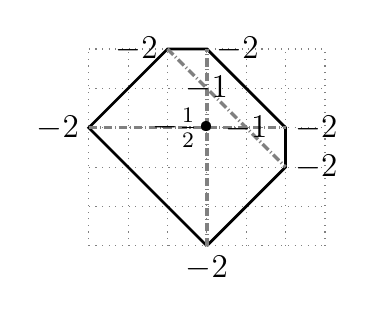
\begin{tikzpicture}[scale=0.5]
 	   \draw[dotted,step=1,gray] (-3,-3) grid (3,2); \draw[line width = 1pt] (0,-3) --
     (-3,0) -- (-1,2)--(0,2)--
 	 (2,0)--(2,-1) -- (0,-3); \draw[densely dashdotted, gray, line width = 1.2pt] (0,-3) -- (0,2);  \draw[densely dashdotted, gray,line width = 1.2pt] (-3,0) -- (2,0); \draw[densely dashdotted, gray,line width = 1.2pt] (-1,2) -- (2,-1);
 	 \node at (0,-3) [below] {\large{$-2$}};
 	 \node at (-3,0) [left] {\large{$-2$}};
 	 \node at (-1,2) [left] {\large{$-2$}};
 	 \node at (0,2) [right] {\large{$-2$}};
 	 \node at (2,0) [right] {\large{$-2$}};
 	 \node at (2,-1) [right] {\large{$-2$}};
 	 \node at (1,0) {\large{$-1$}};
 	 \node at (0,1) {\large{$-1$}};
 	 \node at (0,0) [left] {\large{$-\frac{1}{2}$}};
 	 \draw (0,0) node {\textbullet};
	\end{tikzpicture}
	\caption*{$\deg \Phi $}
\end{subfigure}
}
\end{figure}
\begin{tabularx}{\textwidth}{|c|c|c}
\toprule
\(y\) & \(\text{Vert}(\Delta_y)\) & \(n_y\) \\
\midrule
\(0\) & \begin{tabular}{l} \((-3,0,1),(-2,1,1),(2,1,-1),\) \\ \hspace{1cm} \((3,0,-2),(0,-3,1),(0,1,1)\) \end{tabular} & \((a,b,c)\) \\ \midrule
\(1\) & \begin{tabular}{l} \((-3,0,1),(-2,1,1),(0,1,0),\) \\ \hspace{1cm} \((2,1,1),(3,0,1),(0,-3,-2)\) \end{tabular} & \((a,b,c)\) \\ \midrule
\(\infty\) & \begin{tabular}{l} \((-3,0,-1),(-2,1,-1),(2,1,1),\) \\ \hspace{1cm} \((3,0,2),(0,-3,2),(0,0,-1),(0,1,-1)\) \end{tabular} & \((a,b,c)\) \\
\midrule
\end{tabularx}
\begin{align*}
g(\xi) &= \frac{1}{\xi_{2}^{4}}\cdot\left({\left(2 \, \xi_{2}^{3} - 3 \, \xi_{2} - 3\right)} e^{\left(4 \, \xi_{2}\right)} + 12 \, \xi_{2} e^{\left(3 \, \xi_{2}\right)} + 3 \, \xi_{2} + 3\right) e^{\left(-3 \, \xi_{2}\right)}
\end{align*}
\begin{tabularx}{\textwidth}{|c|c|c}
\toprule
\(y\) & \( h_y(\xi_2)\) & \( h_y(\xi_2) \in\) \\
\midrule
\(0\) & \begin{tabular}{l} \(\frac{1}{3\xi_2^{4}} \cdot
 ( \ (2   \xi_2^{3} - 3   \xi_2 - 3) e^{4   \xi_2} \)   \\ \hspace{2cm} \(+12 \xi_2 e^{3 \xi_2} + 3 \xi_2 + 3 \ ) e^{-3 \xi_2}\) \end{tabular} & \((1.087,1.458)\) \\ \midrule
\(1\) & \begin{tabular}{l} \(\frac{1}{3\xi_2^{4}} \cdot
 ( \ (2   \xi_2^{3} - 3   \xi_2 - 3) e^{4   \xi_2} \)   \\ \hspace{2cm} \(+12 \xi_2 e^{3 \xi_2} + 3 \xi_2 + 3 \ ) e^{-3 \xi_2}\) \end{tabular} & \((2.178,2.470)\) \\ \midrule
\(\infty\) & \begin{tabular}{l} \(\frac{1}{3\xi_2^{4}} \cdot
 ( \ (2   \xi_2^{3} - 3   \xi_2 - 3) e^{4   \xi_2} \)   \\ \hspace{2cm} \(+12 \xi_2 e^{3 \xi_2} + 3 \xi_2 + 3 \ ) e^{-3 \xi_2}\) \end{tabular} & \((0.446,0.827)\) \\ \midrule
\(\notin \{0,1,\infty\}\) & \begin{tabular}{l} \(\frac{1}{3\xi_2^{4}} \cdot
 ( \ (2   \xi_2^{3} - 3   \xi_2 - 3) e^{4   \xi_2} \)   \\ \hspace{2cm} \(+12 \xi_2 e^{3 \xi_2} + 3 \xi_2 + 3 \ ) e^{-3 \xi_2}\) \end{tabular} & \((4.151,4.309)\) \\
 \bottomrule
\end{tabularx}
\newpage
%
%
%
%
%
%
%
%
\begin{figure}[H]
\centering
\label{fig:data318}
\resizebox{0.9\linewidth}{!}{
\begin{subfigure}[b]{0.30\textwidth}
\centering
  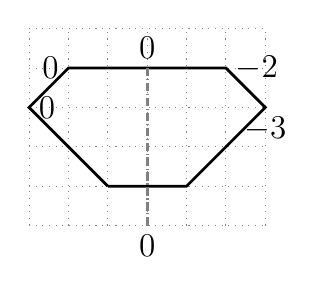
\begin{tikzpicture}[scale=0.5]
   	 \draw[dotted,step=1,gray,] (-3,-3) grid (3,2); \draw[line width = 1pt] (-1,-2) --
     (-3,0) -- (-2,1)--(2,1)--
 	 (3,0)--(1,-2) -- (-1,-2); \draw[densely dashdotted, gray, line width = 1.2pt] (0,-3) -- (0,1);
 	 \node at (0,-3) [below] {\large{$0$}};
 	 \node at (-3,0) [right] {\large{$0$}};
 	 \node at (-2,1) [left] {\large{$0$}};
 	 \node at (2,1) [right] {\large{$-2$}};
 	 \node at (3,0) [below] {\large{$-3$}};
 	 \node at (0,1) [above] {\large{$0$}};
	\end{tikzpicture}
	\caption*{$\Phi_0$}
\end{subfigure}
\begin{subfigure}[b]{0.30\textwidth}
	\centering
 	 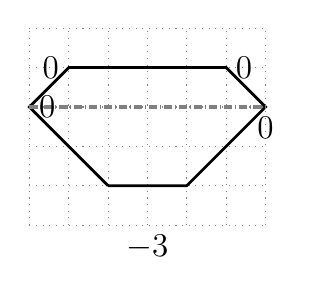
\begin{tikzpicture}[scale=0.5]
 	   \draw[dotted,step=1,gray] (-3,-3) grid (3,2); \draw[line width = 1pt] (-1,-2) --
     (-3,0) -- (-2,1)--(2,1)--
 	 (3,0)--(1,-2) -- (-1,-2); \draw[densely dashdotted, gray,line width = 1.2pt] (-3,0) -- (3,0);
 	 \node at (0,-3) [below] {\large{$-3$}};
 	 \node at (-3,0) [right] {\large{$0$}};
 	 \node at (-2,1) [left] {\large{$0$}};
 	 \node at (2,1) [right] {\large{$0$}};
 	 \node at (3,0) [below] {\large{$0$}};
	\end{tikzpicture}
	\caption*{$\Phi_1$}
\end{subfigure}
\begin{subfigure}[b]{0.30\textwidth}
	\centering
 	 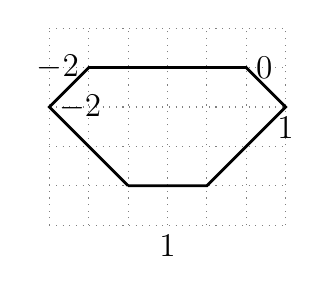
\begin{tikzpicture}[scale=0.5]
 	   \draw[dotted,step=1,gray] (-3,-3) grid (3,2); \draw[line width = 1pt] (-1,-2) --
     (-3,0) -- (-2,1)--(2,1)--
 	 (3,0)--(1,-2) -- (-1,-2);
 	 \node at (0,-3) [below] {\large{$1$}};
 	 \node at (-3,0) [right] {\large{$-2$}};
 	 \node at (-2,1) [left] {\large{$-2$}};
 	 \node at (2,1) [right] {\large{$0$}};
 	 \node at (3,0) [below] {\large{$1$}};
	\end{tikzpicture}
	\caption*{$\Phi_\infty$}
\end{subfigure}
\begin{subfigure}[b]{0.40\textwidth}
	\centering
 	 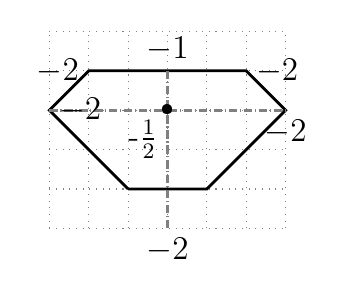
\begin{tikzpicture}[scale=0.5]
 	   \draw[dotted,step=1,gray] (-3,-3) grid (3,2); \draw[line width = 1pt] (-1,-2) --
     (-3,0) -- (-2,1)--(2,1)--
 	 (3,0)--(1,-2) -- (-1,-2); \draw[densely dashdotted, gray,line width = 1.2pt] (-3,0) -- (3,0); \draw[densely dashdotted, gray,line width = 1.2pt] (0,-3) -- (0,1) ;
 	 \node at (0,-3) [below] {\large{$-2$}};
 	 \node at (-3,0) [right] {\large{$-2$}};
 	 \node at (-2,1) [left] {\large{$-2$}};
 	 \node at (2,1) [right] {\large{$-2$}};
 	 \node at (3,0) [below] {\large{$-2$}};
 	 \node at (0,0) [below left] {\large{-$\frac{1}{2}$}};
 	 \node at (0,1) [above] {\large{$-1$}};
 	 \draw (0,0) node {\textbullet};
	\end{tikzpicture}
	\caption*{$\deg \Phi $}
\end{subfigure}
}
\end{figure}

\begin{figure}[h]
\centering
\label{fig:data321}
\resizebox{0.9\linewidth}{!}{
\begin{subfigure}[b]{0.30\textwidth}
\centering
  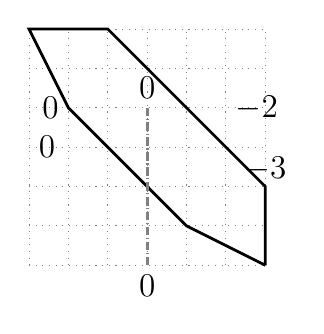
\begin{tikzpicture}[scale=0.5]
   	 \draw[dotted,step=1,gray,] (-3,-3) grid (3,3); \draw[line width = 1pt] (3,-3) --
     (1,-2) -- (-2,1)--(-3,3)--
 	 (-1,3)--(3,-1) -- (3,-3); \draw[densely dashdotted, gray, line width = 1.2pt] (0,-3) -- (0,1);
 	 \node at (0,-3) [below] {\large{$0$}};
 	 \node at (-3,0) [right] {\large{$0$}};
 	 \node at (-2,1) [left] {\large{$0$}};
 	 \node at (2,1) [right] {\large{$-2$}};
 	 \node at (3,0) [below] {\large{$-3$}};
 	 \node at (0,1) [above] {\large{$0$}};
	\end{tikzpicture}
	\caption*{$\Phi_0$}
\end{subfigure}
\begin{subfigure}[b]{0.30\textwidth}
	\centering
 	 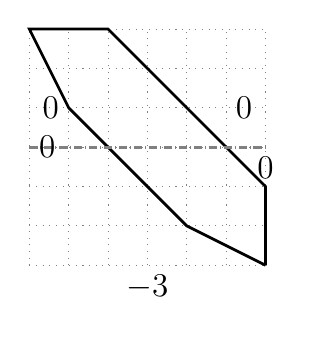
\begin{tikzpicture}[scale=0.5]
   	 \draw[dotted,step=1,gray,] (-3,-3) grid (3,3); \draw[line width = 1pt] (3,-3) --
     (1,-2) -- (-2,1)--(-3,3)--
 	 (-1,3)--(3,-1) -- (3,-3); \draw[densely dashdotted, gray,line width = 1.2pt] (-3,0) -- (3,0);
 	 \node at (0,-3) [below] {\large{$-3$}};
 	 \node at (-3,0) [right] {\large{$0$}};
 	 \node at (-2,1) [left] {\large{$0$}};
 	 \node at (2,1) [right] {\large{$0$}};
 	 \node at (3,0) [below] {\large{$0$}};
	\end{tikzpicture}
	\caption*{$\Phi_1$}
\end{subfigure}
\begin{subfigure}[b]{0.30\textwidth}
	\centering
 	 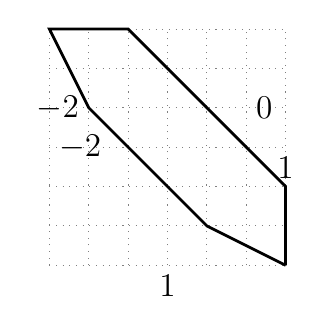
\begin{tikzpicture}[scale=0.5]
   	 \draw[dotted,step=1,gray,] (-3,-3) grid (3,3); \draw[line width = 1pt] (3,-3) --
     (1,-2) -- (-2,1)--(-3,3)--
 	 (-1,3)--(3,-1) -- (3,-3);
 	 \node at (0,-3) [below] {\large{$1$}};
 	 \node at (-3,0) [right] {\large{$-2$}};
 	 \node at (-2,1) [left] {\large{$-2$}};
 	 \node at (2,1) [right] {\large{$0$}};
 	 \node at (3,0) [below] {\large{$1$}};
	\end{tikzpicture}
	\caption*{$\Phi_\infty$}
\end{subfigure}
\begin{subfigure}[b]{0.40\textwidth}
	\centering
 	 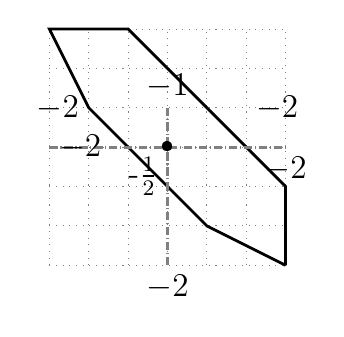
\begin{tikzpicture}[scale=0.5]
   	 \draw[dotted,step=1,gray,] (-3,-3) grid (3,3); \draw[line width = 1pt] (3,-3) --
     (1,-2) -- (-2,1)--(-3,3)--
 	 (-1,3)--(3,-1) -- (3,-3); \draw[densely dashdotted, gray,line width = 1.2pt] (-3,0) -- (3,0); \draw[densely dashdotted, gray,line width = 1.2pt] (0,-3) -- (0,1) ;
 	 \node at (0,-3) [below] {\large{$-2$}};
 	 \node at (-3,0) [right] {\large{$-2$}};
 	 \node at (-2,1) [left] {\large{$-2$}};
 	 \node at (2,1) [right] {\large{$-2$}};
 	 \node at (3,0) [below] {\large{$-2$}};
 	 \node at (0,0) [below left] {\large{-$\frac{1}{2}$}};
 	 \node at (0,1) [above] {\large{$-1$}};
 	 \draw (0,0) node {\textbullet};
	\end{tikzpicture}
	\caption*{$\deg \Phi $}
\end{subfigure}
}
\end{figure}

\begin{figure}[h]
\centering

\label{fig:data322}
\resizebox{0.9\linewidth}{!}{
\begin{subfigure}[b]{0.30\textwidth}
\centering
  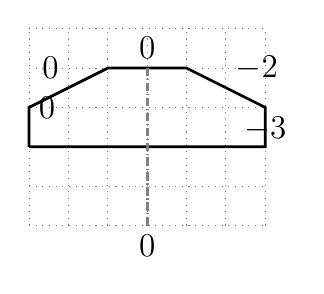
\begin{tikzpicture}[scale=0.5]
   	 \draw[dotted,step=1,gray,] (-3,-3) grid (3,2); \draw[line width = 1pt] (-3,-1) --
     (-3,0) -- (-1,1)--(1,1)--
 	 (3,0)--(3,-1) -- (-3,-1); \draw[densely dashdotted, gray, line width = 1.2pt] (0,-3) -- (0,1);
 	 \node at (0,-3) [below] {\large{$0$}};
 	 \node at (-3,0) [right] {\large{$0$}};
 	 \node at (-2,1) [left] {\large{$0$}};
 	 \node at (2,1) [right] {\large{$-2$}};
 	 \node at (3,0) [below] {\large{$-3$}};
 	 \node at (0,1) [above] {\large{$0$}};
	\end{tikzpicture}
	\caption*{$\Phi_0$}
\end{subfigure}
\begin{subfigure}[b]{0.30\textwidth}
	\centering
 	 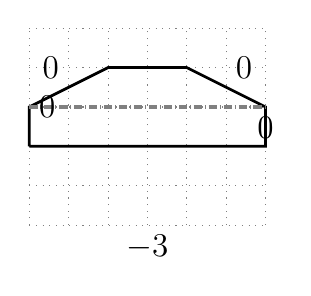
\begin{tikzpicture}[scale=0.5]
 	   \draw[dotted,step=1,gray] (-3,-3) grid (3,2); \draw[line width = 1pt] (-3,-1) --
     (-3,0) -- (-1,1)--(1,1)--
 	 (3,0)--(3,-1) -- (-3,-1); \draw[densely dashdotted, gray,line width = 1.2pt] (-3,0) -- (3,0);
 	 \node at (0,-3) [below] {\large{$-3$}};
 	 \node at (-3,0) [right] {\large{$0$}};
 	 \node at (-2,1) [left] {\large{$0$}};
 	 \node at (2,1) [right] {\large{$0$}};
 	 \node at (3,0) [below] {\large{$0$}};
	\end{tikzpicture}
	\caption*{$\Phi_1$}
\end{subfigure}
\begin{subfigure}[b]{0.30\textwidth}
	\centering
 	 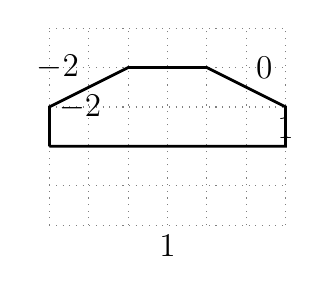
\begin{tikzpicture}[scale=0.5]
 	   \draw[dotted,step=1,gray] (-3,-3) grid (3,2); \draw[line width = 1pt] (-3,-1) --
     (-3,0) -- (-1,1)--(1,1)--
 	 (3,0)--(3,-1) -- (-3,-1);
 	 \node at (0,-3) [below] {\large{$1$}};
 	 \node at (-3,0) [right] {\large{$-2$}};
 	 \node at (-2,1) [left] {\large{$-2$}};
 	 \node at (2,1) [right] {\large{$0$}};
 	 \node at (3,0) [below] {\large{$1$}};
	\end{tikzpicture}
	\caption*{$\Phi_\infty$}
\end{subfigure}
\begin{subfigure}[b]{0.40\textwidth}
	\centering
 	 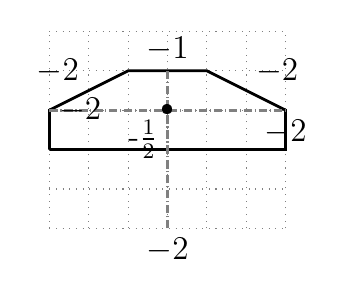
\begin{tikzpicture}[scale=0.5]
 	   \draw[dotted,step=1,gray] (-3,-3) grid (3,2); \draw[line width = 1pt] (-3,-1) --
     (-3,0) -- (-1,1)--(1,1)--
 	 (3,0)--(3,-1) -- (-3,-1); \draw[densely dashdotted, gray,line width = 1.2pt] (-3,0) -- (3,0); \draw[densely dashdotted, gray,line width = 1.2pt] (0,-3) -- (0,1) ;
 	 \node at (0,-3) [below] {\large{$-2$}};
 	 \node at (-3,0) [right] {\large{$-2$}};
 	 \node at (-2,1) [left] {\large{$-2$}};
 	 \node at (2,1) [right] {\large{$-2$}};
 	 \node at (3,0) [below] {\large{$-2$}};
 	 \node at (0,0) [below left] {\large{-$\frac{1}{2}$}};
 	 \node at (0,1) [above] {\large{$-1$}};
 	 \draw (0,0) node {\textbullet};
	\end{tikzpicture}
	\caption*{$\deg \Phi $}
\end{subfigure}
}
\end{figure}

\begin{figure}[h]
\centering
\label{fig:data323}
\resizebox{0.9\linewidth}{!}{
\begin{subfigure}[b]{0.30\textwidth}
\centering
  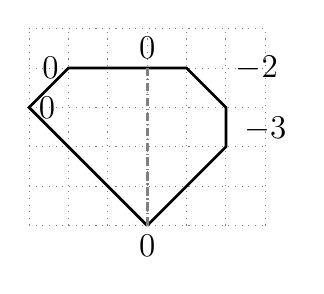
\begin{tikzpicture}[scale=0.5]
   	 \draw[dotted,step=1,gray,] (-3,-3) grid (3,2); \draw[line width = 1pt] (0,-3) --
     (-3,0) -- (-2,1)--(1,1)--
 	 (2,0)--(2,-1) -- (0,-3); \draw[densely dashdotted, gray, line width = 1.2pt] (0,-3) -- (0,1);
 	 \node at (0,-3) [below] {\large{$0$}};
 	 \node at (-3,0) [right] {\large{$0$}};
 	 \node at (-2,1) [left] {\large{$0$}};
 	 \node at (2,1) [right] {\large{$-2$}};
 	 \node at (3,0) [below] {\large{$-3$}};
 	 \node at (0,1) [above] {\large{$0$}};
	\end{tikzpicture}
	\caption*{$\Phi_0$}
\end{subfigure}
\begin{subfigure}[b]{0.30\textwidth}
	\centering
 	 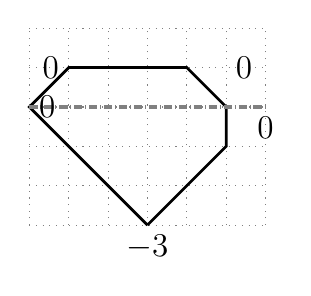
\begin{tikzpicture}[scale=0.5]
 	   \draw[dotted,step=1,gray] (-3,-3) grid (3,2); \draw[line width = 1pt] (0,-3) --
     (-3,0) -- (-2,1)--(1,1)--
 	 (2,0)--(2,-1) -- (0,-3); \draw[densely dashdotted, gray,line width = 1.2pt] (-3,0) -- (3,0);
 	 \node at (0,-3) [below] {\large{$-3$}};
 	 \node at (-3,0) [right] {\large{$0$}};
 	 \node at (-2,1) [left] {\large{$0$}};
 	 \node at (2,1) [right] {\large{$0$}};
 	 \node at (3,0) [below] {\large{$0$}};
	\end{tikzpicture}
	\caption*{$\Phi_1$}
\end{subfigure}
\begin{subfigure}[b]{0.30\textwidth}
	\centering
 	 \begin{tikzpicture}[scale=0.5]
 	   \draw[dotted,step=1,gray] (-3,-3) grid (3,2); \draw[line width = 1pt] (0,-3) --
     (-3,0) -- (-2,1)--(1,1)--
 	 (2,0)--(2,-1) -- (0,-3);
 	 \node at (0,-3) [below] {\large{$1$}};
 	 \node at (-3,0) [right] {\large{$-2$}};
 	 \node at (-2,1) [left] {\large{$-2$}};
 	 \node at (2,1) [right] {\large{$0$}};
 	 \node at (3,0) [below] {\large{$1$}};
	\end{tikzpicture}
	\caption*{$\Phi_\infty$}
\end{subfigure}
\begin{subfigure}[b]{0.40\textwidth}
	\centering
 	 \begin{tikzpicture}[scale=0.5]
 	   \draw[dotted,step=1,gray] (-3,-3) grid (3,2); \draw[line width = 1pt] (0,-3) --
     (-3,0) -- (-2,1)--(1,1)--
 	 (2,0)--(2,-1) -- (0,-3); \draw[densely dashdotted, gray,line width = 1.2pt] (-3,0) -- (3,0); \draw[densely dashdotted, gray,line width = 1.2pt] (0,-3) -- (0,1) ;
 	 \node at (0,-3) [below] {\large{$-2$}};
 	 \node at (-3,0) [right] {\large{$-2$}};
 	 \node at (-2,1) [left] {\large{$-2$}};
 	 \node at (2,1) [right] {\large{$-2$}};
 	 \node at (3,0) [below] {\large{$-2$}};
 	 \node at (0,0) [below left] {\large{-$\frac{1}{2}$}};
 	 \node at (0,1) [above] {\large{$-1$}};
 	 \draw (0,0) node {\textbullet};
	\end{tikzpicture}
	\caption*{$\deg \Phi $}
\end{subfigure}
}
\end{figure}

\begin{figure}[h]
\centering


\label{fig:data324}
\resizebox{0.9\linewidth}{!}{
\begin{subfigure}[b]{0.30\textwidth}
\centering
  \begin{tikzpicture}[scale=0.5]
   	 \draw[dotted,step=1,gray,] (-3,-3) grid (3,2); \draw[line width = 1pt] (0,-2) --
     (-2,0) -- (-2,1)--(1,1)--
 	 (2,0)--(2,-2) -- (0,-2); \draw[densely dashdotted, gray, line width = 1.2pt] (0,-3) -- (0,1);
 	 \node at (0,-3) [below] {\large{$0$}};
 	 \node at (-3,0) [right] {\large{$0$}};
 	 \node at (-2,1) [left] {\large{$0$}};
 	 \node at (2,1) [right] {\large{$-2$}};
 	 \node at (3,0) [below] {\large{$-3$}};
 	 \node at (0,1) [above] {\large{$0$}};
	\end{tikzpicture}
	\caption*{$\Phi_0$}
\end{subfigure}
\begin{subfigure}[b]{0.30\textwidth}
	\centering
 	 \begin{tikzpicture}[scale=0.5]
 	   \draw[dotted,step=1,gray] (-3,-3) grid (3,2); \draw[line width = 1pt] (0,-2) --
     (-2,0) -- (-2,1)--(1,1)--
 	 (2,0)--(2,-2) -- (0,-2); \draw[densely dashdotted, gray,line width = 1.2pt] (-3,0) -- (3,0);
 	 \node at (0,-3) [below] {\large{$-3$}};
 	 \node at (-3,0) [right] {\large{$0$}};
 	 \node at (-2,1) [left] {\large{$0$}};
 	 \node at (2,1) [right] {\large{$0$}};
 	 \node at (3,0) [below] {\large{$0$}};
	\end{tikzpicture}
	\caption*{$\Phi_1$}
\end{subfigure}
\begin{subfigure}[b]{0.30\textwidth}
	\centering
 	 \begin{tikzpicture}[scale=0.5]
 	   \draw[dotted,step=1,gray] (-3,-3) grid (3,2); \draw[line width = 1pt] (0,-2) --
     (-2,0) -- (-2,1)--(1,1)--
 	 (2,0)--(2,-2) -- (0,-2);
 	 \node at (0,-3) [below] {\large{$1$}};
 	 \node at (-3,0) [right] {\large{$-2$}};
 	 \node at (-2,1) [left] {\large{$-2$}};
 	 \node at (2,1) [right] {\large{$0$}};
 	 \node at (3,0) [below] {\large{$1$}};
	\end{tikzpicture}
	\caption*{$\Phi_\infty$}
\end{subfigure}
\begin{subfigure}[b]{0.40\textwidth}
	\centering
 	 \begin{tikzpicture}[scale=0.5]
 	   \draw[dotted,step=1,gray] (-3,-3) grid (3,2); \draw[line width = 1pt] (0,-2) --
     (-2,0) -- (-2,1)--(1,1)--
 	 (2,0)--(2,-2) -- (0,-2); \draw[densely dashdotted, gray,line width = 1.2pt] (-3,0) -- (3,0); \draw[densely dashdotted, gray,line width = 1.2pt] (0,-3) -- (0,1) ;
 	 \node at (0,-3) [below] {\large{$-2$}};
 	 \node at (-3,0) [right] {\large{$-2$}};
 	 \node at (-2,1) [left] {\large{$-2$}};
 	 \node at (2,1) [right] {\large{$-2$}};
 	 \node at (3,0) [below] {\large{$-2$}};
 	 \node at (0,0) [below left] {\large{-$\frac{1}{2}$}};
 	 \node at (0,1) [above] {\large{$-1$}};
 	 \draw (0,0) node {\textbullet};
	\end{tikzpicture}
	\caption*{$\deg \Phi $}
\end{subfigure}
}
\end{figure}

%\begin{figure}[h]
%\centering
%
%\label{fig:data45*}
%\resizebox{0.9\linewidth}{!}{
%\begin{subfigure}[b]{0.30\textwidth}
%\centering
%  \begin{tikzpicture}[scale=0.5]
%   	 \draw[dotted,step=1,gray,] (-3,-3) grid (3,3); \draw[line width = 1pt] (3,-3) --
%     (1,-2) -- (-2,1)--(-3,3)--
% 	 (-2,3)--(3,-2) -- (3,-3); \draw[densely dashdotted, gray, line width = 1.2pt] (0,-3) -- (0,1);
% 	 \node at (3,-3) [below] {\large{$-2$}};
% 	 \node at (1,-2) [right] {\large{$0$}};
% 	 \node at (-2,1) [left] {\large{$0$}};
% 	 \node at (-3,3) [right] {\large{$0$}};
% 	 \node at (-2,3) [right] {\large{$-2$}};
% 	 \node at (3,-2) [right] {\large{$-2$}};
%	\end{tikzpicture}
%	\caption*{$\Phi_0$}
%\end{subfigure}
%\begin{subfigure}[b]{0.30\textwidth}
%	\centering
% 	 \begin{tikzpicture}[scale=0.5]
% 	   \draw[dotted,step=1,gray] (-3,-3) grid (3,3); \draw[line width = 1pt] (3,-3) --
%     (1,-2) -- (-2,1)--(-3,3)--
% 	 (-2,3)--(3,-2) -- (3,-3); \draw[densely dashdotted, gray,line width = 1.2pt] (-3,0) -- (3,0);
% 	 \node at (3,-3) [below] {\large{$-2$}};
% 	 \node at (1,-2) [right] {\large{$0$}};
% 	 \node at (-2,1) [left] {\large{$0$}};
% 	 \node at (-3,3) [right] {\large{$0$}};
% 	 \node at (-2,3) [right] {\large{$-2$}};
% 	 \node at (3,-2) [right] {\large{$-2$}};
%	\end{tikzpicture}
%	\caption*{$\Phi_1$}
%\end{subfigure}
%\begin{subfigure}[b]{0.30\textwidth}
%	\centering
% 	 \begin{tikzpicture}[scale=0.5]
% 	   \draw[dotted,step=1,gray] (-3,-3) grid (3,3); \draw[line width = 1pt] (3,-3) --
%     (1,-2) -- (-2,1)--(-3,3)--
% 	 (-2,3)--(3,-2) -- (3,-3);
% 	 \node at (3,-3) [below] {\large{$-2$}};
% 	 \node at (1,-2) [right] {\large{$0$}};
% 	 \node at (-2,1) [left] {\large{$0$}};
% 	 \node at (-3,3) [right] {\large{$0$}};
% 	 \node at (-2,3) [right] {\large{$-2$}};
% 	 \node at (3,-2) [right] {\large{$-2$}};
%	\end{tikzpicture}
%	\caption*{$\Phi_\infty$}
%\end{subfigure}
%\begin{subfigure}[b]{0.40\textwidth}
%	\centering
% 	 \begin{tikzpicture}[scale=0.5]
% 	   \draw[dotted,step=1,gray] (-3,-3) grid (3,3); \draw[line width = 1pt] (3,-3) --
%     (1,-2) -- (-2,1)--(-3,3)--
% 	 (-2,3)--(3,-2) -- (3,-3); \draw[densely dashdotted, gray,line width = 1.2pt] (0,-1) -- (2,-1); \draw[densely dashdotted, gray,line width = 1.2pt] (-1,0) -- (-1,2) ; \draw[densely dashdotted, gray,line width = 1.2pt] (3,-3) -- (-3,3)
% 	 \node at (3,-3) [right] {\large{$-2$}};
% 	 \node at (1,-2) [below] {\large{$0$}};
% 	 \node at (-2,1) [left] {\large{$0$}};
% 	 \node at (-3,3) [left] {\large{$0$}};
% 	 \node at (-2,3) [above] {\large{$-2$}};
% 	 \node at (3,-2) [right] {\large{$-2$}};
% 	 \node at (2,-1) [right] {\large{$-\frac{3}{2}$}};
% 	 \node at (0,-1) [below left] {\large{$-\frac{3}{2}$}};
% 	 \node at (-1,2) [above] {\large{$-\frac{3}{2}$}};
% 	 \node at (-1,0) [left] {\large{$-\frac{3}{2}$}};
% 	 \draw (0,0) node {\textbullet};
%	\end{tikzpicture}
%	\caption*{$\deg \Phi $}
%\end{subfigure}
%}
%\end{figure}

\begin{figure}[h]
\centering


\label{fig:data48}
\resizebox{0.9\linewidth}{!}{
\begin{subfigure}[b]{0.30\textwidth}
\centering
  \begin{tikzpicture}[scale=0.5]
   	 \draw[dotted,step=1,gray,] (-3,-2) grid (3,2); \draw[line width = 1pt] (-2,-1) --
     (-2,0) -- (-1,1)--(1,1)--
 	 (2,0)--(2,-1) -- (-2,-1); \draw[densely dashdotted, gray, line width = 1.2pt] (0,-1) -- (0,1);
 	 \node at (-2,-1) [left] {\large{$-2$}};
 	 \node at (-2,0) [left] {\large{$-2$}};
 	 \node at (-1,1) [left] {\large{$-1$}};
 	 \node at (0,1) [above] {\large{$0$}};
 	 \node at (1,1) [right] {\large{$0$}};
 	 \node at (2,0) [right] {\large{$0$}};
 	 \node at (2,-1) [right] {\large{$0$}};
 	 \node at (0,-1) [below] {\large{$0$}};
 	 \draw (0,0) node {\textbullet};
	\end{tikzpicture}
	\caption*{$\Phi_0$}
\end{subfigure}
\begin{subfigure}[b]{0.30\textwidth}
	\centering
 	 \begin{tikzpicture}[scale=0.5]
 	   \draw[dotted,step=1,gray] (-3,-2) grid (3,2); \draw[line width = 1pt] (-2,-1) --
     (-2,0) -- (-1,1)--(1,1)--
 	 (2,0)--(2,-1) -- (-2,-1); \draw[densely dashdotted, gray,line width = 1.2pt] (0,-1) -- (0,1); 
 	 \node at (-2,-1) [left] {\large{$0$}};
 	 \node at (-2,0) [left] {\large{$0$}};
 	 \node at (-1,1) [left] {\large{$0$}};
 	 \node at (0,1) [above] {\large{$0$}};
 	 \node at (1,1) [right] {\large{$-1$}};
 	 \node at (2,0) [right] {\large{$-2$}};
 	 \node at (2,-1) [right] {\large{$-2$}};
 	 \node at (0,-1) [below] {\large{$0$}};
 	 \draw (0,0) node {\textbullet};
	\end{tikzpicture}
	\caption*{$\Phi_1$}
\end{subfigure}
\begin{subfigure}[b]{0.30\textwidth}
	\centering
 	 \begin{tikzpicture}[scale=0.5]
 	   \draw[dotted,step=1,gray] (-3,-2) grid (3,2); \draw[line width = 1pt] (-2,-1) --
     (-2,0) -- (-1,1)--(1,1)--
 	 (2,0)--(2,-1) -- (-2,-1); \draw[densely dashdotted, gray,line width = 1.2pt] (-2,0) -- (2,0) ;
 	 \node at (-2,-1) [left] {\large{$0$}};
 	 \node at (-2,0) [left] {\large{$0$}};
 	 \node at (-1,1) [left] {\large{$-1$}};
 	 \node at (0,1) [above] {\large{$-1$}};
 	 \node at (1,1) [right] {\large{$0$}};
 	 \node at (2,0) [right] {\large{$0$}};
 	 \draw (0,0) node {\textbullet};
	\end{tikzpicture}
	\caption*{$\Phi_\infty$}
\end{subfigure}
\begin{subfigure}[b]{0.40\textwidth}
	\centering
 	 \begin{tikzpicture}[scale=0.5]
 	   \draw[dotted,step=1,gray] (-3,-2) grid (3,2); \draw[line width = 1pt] (-2,-1) --
     (-2,0) -- (-1,1)--(1,1)--
 	 (2,0)--(2,-1) -- (-2,-1); \draw[densely dashdotted, gray,line width = 1.2pt] (-2,0) -- (2,0); \draw[densely dashdotted, gray,line width = 1.2pt] (0,-1) -- (0,1) ;
 	 \node at (-2,-1) [left] {\large{$-2$}};
 	 \node at (-2,0) [left] {\large{$-2$}};
 	 \node at (-1,1) [left] {\large{$-2$}};
 	 \node at (0,1) [above] {\large{$-1$}};
 	 \node at (1,1) [right] {\large{$-2$}};
 	 \node at (2,0) [right] {\large{$-2$}};
 	 \node at (2,-1) [right] {\large{$-2$}};
 	 \node at (0,-1) [below] {\large{$0$}};
  	 \node at (0,0) [right] {\large{$0$}};
 	 \draw (0,0) node {\textbullet};
	\end{tikzpicture}
	\caption*{$\deg \Phi $}
\end{subfigure}
}
\end{figure}

}